\chapter{Analyse de robustesse dans le cadre d'injection de fautes multiples}
\chaptermark{Analyse de robustesse pour l'injection multi-fautes} % Header overflow
\label{chpt:background}

    \setcounter{tocdepth}{2}
    \section*{Table des Matières}
    \localtableofcontents
    
    \section{Attaques physiques et injection de fautes}
    \label{sec:physical-attacks}
    
        \subsection{Fautes matérielles aléatoires}
        
            En 1954, Isaac Azimov, un écrivain américain réputé pour ses écrits en science-fiction, publie le livre \og Les cavernes de l'acier \fg{} (dans son titre original \og The Caves of Steel \fg{} \cite{Asimov/Cave}), dans lequel un robot se voit désactivé par le rayonnement d'une particule alpha\footnote{Les particules alpha sont des rayonnements issus de la radioactivité.}. 
            
            Vingt ans plus tard, en 1975, Binder et al. \cite{binder1975satellite} indiquent que les anomalies électroniques observées sur les satellites de télécommunications pourraient être liées aux rayonnements ionisants issus du soleil provoquant le déclenchement de bascules. En 1978, May et al. \cite{May/78} découvrent que des erreurs de valeurs dans la mémoire dynamique \gls{dram}, appelées \textit{soft errors}, peuvent être causées par le rayonnement de particules alpha de l'environnement immédiat des cellules mémoires. 
            
            La problématique de la tolérance aux fautes (\textit{fault tolerance)} face aux corruptions silencieuses de la mémoire (\gls{sdc}) liées à des phénomènes physiques tels que les rayonnements cosmiques \cite{Ziegler/79}, est d'autant plus présente de nos jours en raison de la forte augmentation des tailles de stockages \cite{Charyyev/19}, ou des systèmes hautes performances (\gls{hpc}) \cite{di2016adaptive}. 
            
            Cela a donné lieu à la mise en place d'outils d'analyse de tolérance des programmes aux fautes matérielles \cite{Segall/FTCS88, Kanawati/FTCS92} ainsi que des mécanismes de protection au niveau logiciel ou matériel (comme le déploiement de codes correcteurs d'erreur ou de redondance des données par exemple \cite{Wu/17}). 
            Les années 90 voient émerger l'injection de fautes \cite{karlsson1994using, clark1995fault}, une technique visant à injecter volontairement des fautes dans un système afin d'observer leurs effets sur un composant. Ces injections sont réalisées en induisant un stress sur le système visé à l'aide de radiations d'ions lourds ou de perturbations de l'alimentation par exemple.
            
        \subsection{Attaques par canaux auxiliaires}
            
            En 1996, Korsher et al. \cite{Kocher/96TA} présentent une attaque sur certains crypto-systèmes tels que RSA \cite{Rivest/78RSA} et Diffie-Hellman \cite{Diffie/76}. Ils parviennent à trouver des secrets via l'information que laisse fuiter l'implémentation (sans attaque). Ils confirment ainsi qu'il est possible de profiter des différences dans le temps d'exécution de ces algorithmes pour retrouver les clefs de chiffrement secrètes.
            Ces attaques visant à obtenir de l'information secrète dans une implémentation à l'aide de l'étude de paramètres physiques sont nommées \textit{attaques par canaux auxiliaires} (\textit{side-chanel attacks}), ou attaques par canaux cachés. 
            
            Par la suite, les attaques par canaux auxiliaires se sont étendues à l'analyse de la consommation électrique (\gls{dpa}) \cite{Kocher/99DPA, Korcher/11}, du cache du processeur \cite{Tiri/DAC07}, des rayonnements électromagnétiques \cite{Pandolfi/CHES01} ou encore des ondes sonores telles que celles émises par un clavier \cite{Asonov/SSP04, Gupta/JCS18}.
            L'existence de telles attaques implique la nécessité que l'analyse de sécurité d'un système prenne en compte ce type d'objectifs d'attaque. 
            
        \subsection{Attaques par injection de fautes}
            
            En 1997, Boneh et al. \cite{Boneh/EUROCRYPT97} présentent un modèle théorique permettant de casser des implémentations de crypto-systèmes. Prenant pour appui l'existence de fautes matérielles, ils proposent d'injecter volontairement des fautes pour casser l'implémentation des algorithmes cryptographiques \gls{rsa}, Fiat-Shamir \cite{Fiat/86} et Schnorr \cite{Schnorr/JC91}.
            L'année suivante, Biham et al. \cite{Biham/AICC97} utilisent le terme de \gls{dfa} pour qualifier une attaque reposant sur l'injection volontaire de fautes afin de comparer une exécution normale à des exécutions fautées. Ils parviennent à récupérer la clef secrète d'une implémentation sur carte-à-puce de l'algorithme de chiffrement \gls{des} à l'aide de l'étude comparative d'un chiffré obtenu à partir d'un clair inconnu et de différents chiffrés dont le calcul a été fauté par la modification d'un bit. Ils proposent également une méthodologie pour appliquer ce type d'attaque. La \gls{dfa} est une attaque par canaux auxiliaires \textit{active} (où l'attaquant interagit avec le matériel cible).
            
            Dans les décennies suivantes, plusieurs techniques d'injection de fautes sont apparues: modification de la fréquence de l'horloge \cite{Agoyan/SCRAA10, Yuce/HSS18}, impulsion électromagnétiques \cite{Poucheret/FDTC11}, rayon de lumière \cite{Skorobogatov/CHES02} et faisceaux lasers \cite{Roscian/FDTC13, Colombier/HOST19} par exemple. Chaque méthode possède des caractéristiques spécifiques en ce qui concerne la difficulté et le coût de mise en place, la précision, la reproductibilité et l'effet des fautes \cite{BarEl/IEEE06}.
            
            \begin{sloppypar}   
            Les exploitations de l'injection de fautes ont montré la possibilité d'obtenir des données secrètes d'un algorithme cryptographique \cite{Boneh/JC01, Biham/AICC97}, l'élévation de privilèges \cite{Timmers/FDTC16}, l'introduction de vulnérabilité par dépassement de tampon \cite{Nashimoto/JCE17, SSTIC20} ou bien encore l'évitement d'un boot sécurisé \cite{Nashimoto/JCE17} ou du module d'exécution de confiance \cite{Nashimoto/IACR22}. Des techniques d'injection au niveau logiciel ont aussi été développées, comme par exemple \textit{RowHammer} \cite{Park/IIRW14} qui vise à induire un changement d'une cellule \gls{dram} en actualisant de façon répétée les lignes adjacentes. 
            \end{sloppypar}   
            
        \subsection{Plan du chapitre}
            
            Cette thèse vise l'aide à la conception d'applications robustes contre les attaques par injections de fautes, qui constituent une menace importante pour la sécurité des composants sensibles.
            Il s'agit à la fois de l'aide au développeur et à l'auditeur qui évalue la robustesse de l'application. C'est pourquoi les contributions de cette thèse se concentrent majoritairement sur le niveau logiciel (code source, représentation intermédiaire et assembleur), pour s'intéresser aux fautes mettant en cause la logique algorithmique des implémentations.
            L'objectif de ce chapitre est d'introduire les problématiques liées aux attaques par injection de fautes multiples et à leurs évaluation.
            La section \ref{sec:models} définit les concepts de fautes et de modèles de faute et présente un panorama des modèles considérés afin de présenter les enjeux liés à la modélisation des fautes et de leur propagation au sein d'un système. 
            La section \ref{sec:fi-protections} discute brièvement de la problématique de la mise en place de contre-mesures dans le cadre d'attaques en faute, ce qui sera détaillé dans le chapitre \ref{chpt:ccpo}.
            La section \ref{sec:multi-fault} se penche sur les problématiques posées par les fautes multiples, c'est-à-dire lorsque l'attaquant est capable d'injecter plusieurs fautes lors de son attaque. 
            La section \ref{sec:soa-tools} discute des différentes méthodes et outils utilisés pour l'analyse de robustesse dans le contexte de l'injection de fautes.
        
    \section{Fautes et modèles de faute}
    \label{sec:models}
    
        Un \textit{modèle de faute} correspond au \textit{modèle d'action} du modèle d'attaquant (section \ref{sec:model-attack}), instancié au contexte des attaques par injection de fautes. Il représente l'ensemble des fautes qu'un attaquant est capable de réaliser dans le modèle.
        La notion de \textit{faute} est directement liée au niveau de représentation considéré. 
        Au niveau du code source d'un programme par exemple, les modèles de faute considérés correspondent à des abstractions des effets qu'une faute à plus bas niveau peut avoir sur le programme (par exemple modifier une valeur dans une variable ou changer un branchement). 
        
        Cette section vise à présenter les modèles de faute communément considérés aux différents niveaux de représentation en se concentrant sur les modèles au niveau logiciel.
        La section \ref{sec:abstraction-level-fault} présente une classification des niveaux de représentation et discute des caractéristiques d'une faute et des problématiques de mise en relation des modèles de faute à des niveaux variables.
        La section \ref{sec:soa-models} donne un aperçu des modèles de faute issus des attaques par injection de fautes et de l'analyse de robustesse.
        Enfin, la section \ref{sec:model-classification} discute de la classification des modèles de faute. 
        
        \subsection{Niveaux de représentation et caractéristiques des fautes}
        \label{sec:abstraction-level-fault}
        
            Une \textit{faute} est une modification de l'état du système entraînant un effet sur son comportement. Celle-ci peut-être induite par une injection physique, une injection logicielle ou encore une erreur aléatoire.
            Différents niveaux de représentation sont considérés lorsqu'il s'agit d'analyser un programme ou d'appliquer des protections: au niveau logiciel (langage C, représentation intermédiaire ou assembleur), niveau micro-architectural (\gls{rtl}, \gls{vhdl}), au niveau matériel (technique d'injection physique utilisée) ou encore l'analyse d'un automate représentant le programme par exemple.
            
            La figure \ref{fig:abstraction-level} présente la terminologie qui sera utilisée dans la suite de ce manuscrit en ce qui concerne les niveaux de représentation.
            Les niveaux sont ici organisés en partant du niveau le plus bas (niveau physique) au niveau le plus haut (niveau algorithmique).
            Le \textit{niveau physique} correspond à la perturbation physique déclenchant le comportement fauté, que celle-ci soit liée à une erreur aléatoire, une injection de faute physique ou encore déclenchée par des moyens logiciels.
            Cette injection se traduit au \textit{niveau du circuit} sur les portes logiques, les bascules et latches ou les cellules mémoires et se manifeste en fonction de la partie du système visé, au niveau \textit{micro-architectural} en ciblant une modification des données, des instructions ou de parties spécifiques du processeur par exemple.
            A plus haut niveau, formant le \textit{niveau logiciel}, les fautes sont observables au niveau binaire, au niveau assembleur et au niveau source qui se rapprochent davantage de la logique algorithmique ou des propriétés logiques attendues par la spécification.
            
            \begin{figure}[ht]\centering
              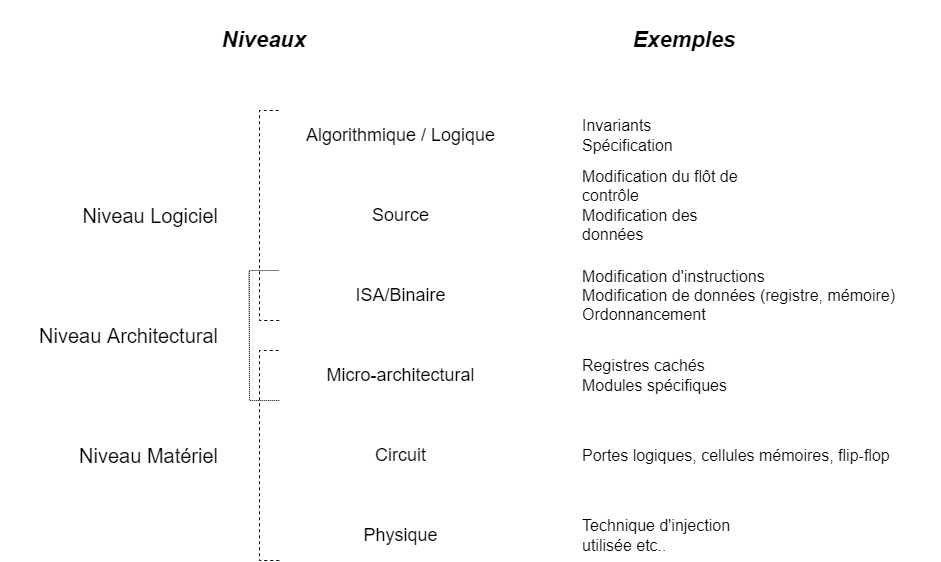
\includegraphics[scale=.43]{ch2-background/img/Modeles all.drawio.png}
              \caption{Classification et terminologie des niveaux de représentation}
              \label{fig:abstraction-level}
            \end{figure}
            
            Chaque niveau de représentation dispose d'avantages et d'inconvénients en ce qui concerne la représentativité du modèle étudié, la facilité de mise en place ou la facilité avec lesquels les résultats peuvent être observés. Un modèle plus haut niveau sera plus générique, plus proche des propriétés logiques de la spécification, tandis qu'un modèle bas niveau sera plus proche de l'effet des techniques d'injections de fautes.   
        
            La manière dont les fautes sont propagées aux travers des différents niveaux n'est pas toujours bien comprise. 
            Observer l'effet d'une faute à un niveau supérieur n'est pas forcément évident.
            L'effet de la faute peut se perdre, par exemple une modification de donnée qui aurait lieu juste avant une réécriture de cette variable passerait inaperçue (schéma \gls{wwr}, aussi appelé \textit{faute inactive}), et les techniques d'injection de fautes peuvent avoir des taux de reproductibilité assez bas.
            Observer l'effet des fautes est donc une problématique à part entière et la caractérisation des modèles de faute vise à comprendre l'effet des fautes et leur propagation aux niveaux suivants \cite{Balasch/FDTC11, Dureuil/CARDIS15, werner2020end}.             
            
            Le \textit{modèle de faute} est donc une spécification de l'ensemble des fautes qu'on autorise à l'attaquant et revient à décrire quelles sont les caractéristiques des fautes qui sont acceptées par le modèle.
            L'\textit{effet de la faute} est une caractéristique des fautes mais d'autres caractéristiques peuvent être considérées. En particulier la \textit{persistance temporelle} (\textit{combien de temps la faute a un impact sur le programme ?}) et la \textit{position spatio-temporelle} (\textit{où et quand la faute est injectée ?}). Pareillement, ces caractéristiques ont un sens qui dépend du niveau de représentation considéré.
            
            \subsubsection{Position spatio-temporelle d'une faute}
            
                Au niveau physique, une faute peut être caractérisée par sa position spatiale (\textit{où la faute est injectée ?}) et sa position temporelle (\textit{quand la faute est injectée ?}). En fonction de la technique d'injection utilisée, la position peut correspondre sur le composant à une entrée physique (tension d'alimentation ou fréquence d'horloge) ou à des bits dans des cellules mémoires ou un bus par exemple.
                La position temporelle correspond au moment où l'injection est effectuée, par exemple compté depuis le démarrage de l'exécution.
                
                A plus haut niveau, ces deux notions peuvent être plus difficiles à distinguer. Au niveau source par exemple, la position de la faute peut correspondre à un point de contrôle du programme, appelé alors \textit{point d'injection} (\gls{ip}). Le listing \ref{lst:inj-point} présente les points d'injection dans une fonction \texttt{compare} avec un modèle de faute permettant à l'attaquant d'inverser le résultat d'une condition. Durant l'exécution, $IP1$ et $IP2$ peuvent se déclencher, c'est-à-dire qu'une faute peut y être injectée à chaque exécution de boucle. 
            
\lstset{caption={Points d'injection pour la fonction \texttt{compare}},label=lst:inj-point}
\begin{lstlisting}     
bool compare(uint8_t* a1, uint8_t* a2, size_t size)
{
    bool result = true;
    for(size_t i = 0; i < size; i++) { // IP1
        if(a1[i] != a2[i]) { // IP2
            result = false;
        }
    }
    return result;
}
\end{lstlisting}            

                On appellera l'\textit{espace de faute} l'ensemble des points d'injection sur un programme pour un modèle de faute donné. La figure \ref{fig:soft-hard-compare} présente l'espace des fautes pour le modèle d'inversion de test logiciel, ainsi que l'espace des fautes d'un modèle au niveau physique permettant d'obtenir un comportement d'inversion de test, par exemple en ciblant le registre contenant le résultat de la condition lors des évaluations des tests. Les fautes sont ici les mêmes mais sont caractérisées par un ensemble de points d'injection dans le cas du modèle au niveau logiciel et par les paramètres de l'injection au niveau physique.
                
                \begin{figure}
                  \makebox[\textwidth][c]{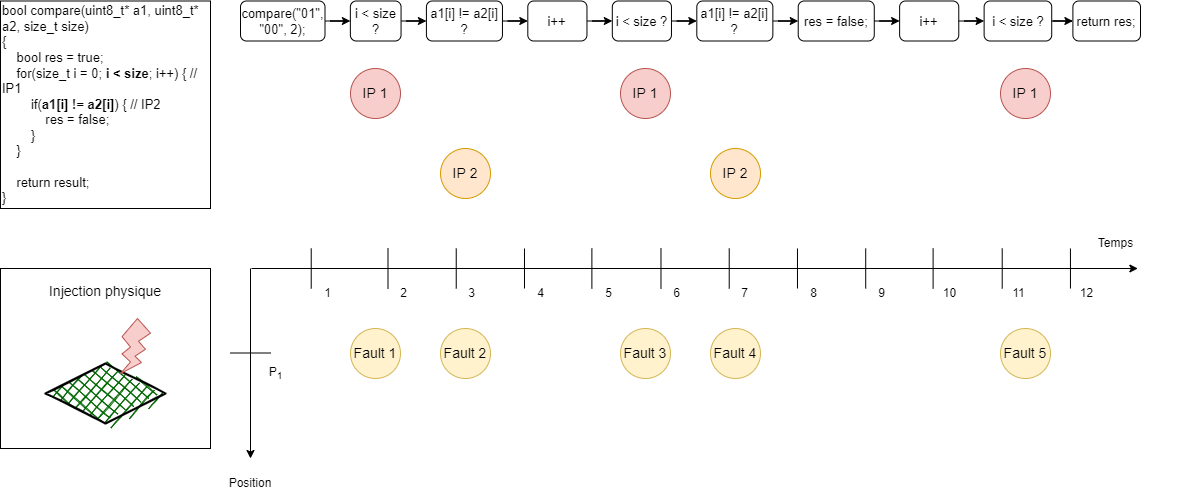
\includegraphics[scale=.41]{ch2-background/img/spatiotemporal.drawio.png}}
                  \caption{Comparaison des fautes sur la fonction compare en inversion de test}
                  \label{fig:soft-hard-compare}
                \end{figure}            
        
            \subsubsection{Persistance temporelle}
                
                BarEl et al. \cite{BarEl/IEEE06} indiquent qu'un circuit peut être sujet à deux types de fautes: les fautes \textbf{permanentes} (destructives) et les fautes \textbf{transitoires}.
                Dans le cas de fautes \textit{transitoires} (ou \textit{provisoires}), la faute a un effet immédiat sur le système en provoquant une mauvaise interprétation d'un signal. Lorsque la faute cesse, le circuit revient ensuite à son état initial.
                A l'inverse, les fautes \textit{destructives} ont un effet permanent sur le système en altérant l'intégrité d'un registre, d'une cellule mémoire ou du circuit par exemple.
                
                En pratique, cette taxonomie au niveau physique est difficile à transposer à un niveau d'abstraction plus élevé. Une faute transitoire peut avoir un effet \textit{permanent} ou \textit{semi-permanent}, sur le programme.
                Par exemple, si une faute transitoire modifie une valeur dans un registre qui est ensuite écrite en mémoire vive (\gls{ram}), alors l'effet de la faute persistera jusqu'à la fin de l'exécution du programme. Dans sa thèse \cite{Brejon/Phd20}, J.-B. Bréjon parle de \textbf{faute persistante} lorsque qu'une faute transitoire a un effet qui persiste au delà de son effet physique sur le circuit. Il cite aussi le cas où une faute transitoire implique une modification d'une instruction du programme chargée en \gls{ram}.
                Dans un cas plus extrême, une faute transitoire peut avoir un effet permanent sur un système, par exemple si la valeur fautée est ensuite utilisée dans un système de mise à jour de micro-programme (firmware updater). La faute aura alors un impact sur le système même après la fin de l'exécution du programme, voire provoquera l'arrêt du système, la faute ayant été répercutée dans la mémoire non volatile.
                On parle aussi de fautes \textit{transitoires répétitives} \cite{Berthome/ARES12} lorsqu'une faute transitoire peut être répétée, par exemple en fautant un bus mémoire plusieurs fois pour introduire plusieurs valeurs invalides successivement.
            
        \subsection{État de l'art des modèles de faute}
        \label{sec:soa-models}
        
            Cette sous-section propose un aperçu des modèles de faute considérés dans la littérature, à la fois par les attaques physiques et par les outils d'analyse. Cet état de l'art est organisé en fonction du niveau de représentation du programme.
            La section \ref{sec:model:physic} présente les modèles au niveau matériel, la section \ref{sec:model:binary} les modèles de faute au niveau de la micro-architecture et du jeu d'instructions, ainsi que des modèles au niveau assembleur et finalement la section \ref{sec:model:source} se concentre sur les modèles au niveau source.
        
            \subsubsection{Modèles au niveau matériel}
            \label{sec:model:physic}
            
                Au niveau physique, l'injection d'une faute introduit une perturbation qui va modifier le fonctionnement du circuit. Le circuit peut consister en des portes logiques, des cellules mémoire ou encore des bascules.
                
                Le modèle de faute considéré à bas niveau est lié à la technique d'injection de fautes utilisée. Certaines techniques comme celles basées sur les ondes électromagnétiques \cite{Maistri/VLSI-SoC14, Dument/FDTC19} ou les impulsions laser \cite{Van/FDTC11, Dutertre/DTIS14} ont une haute précision à l'inverse des glitchs de température \cite{Hutter/ICSCRAA13} par exemple.
                Les caractéristiques des fautes injectées vont alors dépendre des paramètres expérimentaux choisis (moment et position de l'injection, durée et intensité d'un rayonnement etc.).
                
                \begin{table}[ht]
                \centering
                    \begin{tabular}{|l|l|l|l|}
                    \hline
                    Valeur / Granularité & Niveau bit & Niveau byte & Autres plages \\ \hline \hline
                    mise à 0                             & bit-set       & byte set        & set          \\ \hline
                    mise à 1                             & bit-reset     & byte reset      & reset        \\ \hline
                    inversion                            & bit flip   & byte flip       & flip         \\ \hline
                    aléatoire                            & bit ran    & byte ran       & rand    \\    \hline
                    \end{tabular}               
                \caption{Modèle de faute sur les données \label{tbl:bits}}
                \end{table}
                
                Au niveau d'une donnée dans le circuit (dans un bus ou une cellule mémoire par exemple), on distingue souvent les modèles en fonction de la granularité de la plage de bits pouvant être visée et la façon dont la valeur peut être modifiée, comme indiqué dans la table \ref{tbl:bits}.
                La granularité de la faute en donnée peut consister en un seul bit, un octet, une plage contiguë quelconque ou une plage non contiguë de bits.
                Concernant la valeur fautée, on peut distinguer les modèles de mise-à-zéro et de mise-à-un ainsi que l'inversion des bits. 
                Les modèles de type aléatoire permettent de simuler les injections en données sur des mémoires chiffrées où l'attaquant a un contrôle limité sur la valeur qui pourra être injectée. 
            
            \subsubsection{Modèles au niveau architectural et ISA}
            \label{sec:model:binary}
            
                Au niveau architectural, les fautes peuvent être distinguées en fonction de la partie de l'architecture qui est ciblée comme présenté dans la figure \ref{fig:arch-models-scheme}:
                \begin{itemize}
                    \item fautes sur les instructions,
                    \item fautes sur les données (registres, cache, mémoire),
                    \item fautes sur la micro-architecture: pipeline, registres cachés...
                \end{itemize}             
                
                \begin{figure}[ht]
                    \centering
                    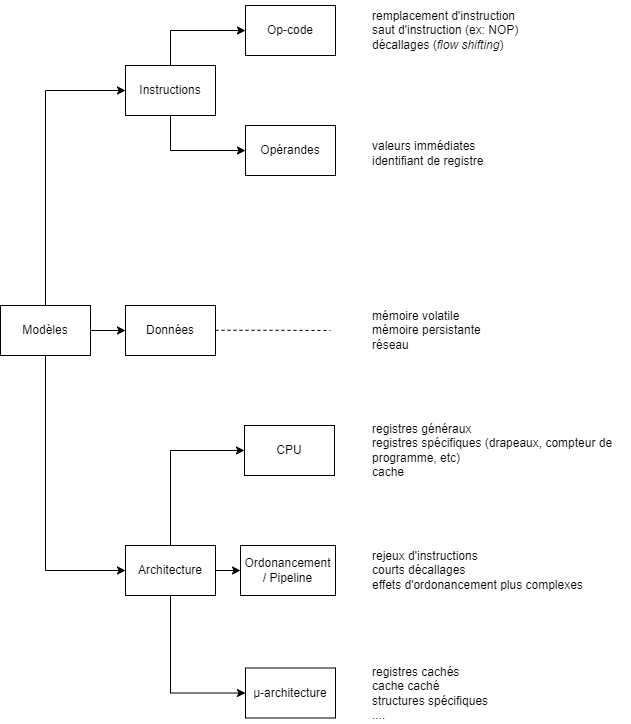
\includegraphics[scale=.56]{ch2-background/img/Modeles Architecture fr.drawio.png}
                    \caption{Classification des modèles au niveau architectural}
                    \label{fig:arch-models-scheme}
                \end{figure}
                    
                \paragraph{}
                Lorsqu'on se place au niveau du jeu d'instructions (\gls{isa}), une modification de bits induit une transformation des instructions ou des données.
                Une faute peut avoir pour effet la modification de l'opérande (les paramètres de l'instruction), de l'opcode (le type de l'instruction) ou les deux.
                
                La figure \ref{fig:armv7-mov-encoding} présente la spécification de l'encodage des trois versions de l'instruction \textit{MOV} dans le jeu d'instructions \textit{ARMv7-M thumb2} \cite{ARMv7/manual}. 
                Les bits correspondant à l'opcode dans l'encodage sont indiqués avec une valeur fixe binaire tandis que les opérandes sont nommées. Les opérandes de la forme \texttt{immX} correspondent à la valeur immédiate (constante) qui sera déplacée et \texttt{rd} correspond au registre de destination. Si ces bits sont changés par une faute, le type de l'instruction restera le même (MOV-TX), mais avec des paramètres différents \cite{Colombier/HOST19}.
                Un cas particulier du remplacement d'instruction est le saut d'instructions\footnote{D'autres types de fautes peuvent toutefois induire un saut d'instruction, comme par exemple la modification du compteur du programme (\gls{pc}).} très largement étudié \cite{Balasch/FDTC11, Kelly/HOST17, Moro/FDTC13}, dans lequel la faute permet d'ignorer l'exécution d'une ou plusieurs instructions (par exemple, en transformant une instruction en instruction \gls{nop})).
                Dans le cas de jeu d'instructions à taille d'instruction variable comme c'est le cas pour \textit{thumb}, la mutation au niveau de l'\textit{op-code} peut jouer sur la taille de l'instruction (en passant d'une instruction de deux à quatre octets ou réciproquement) et peut entraîner une mutation en cascade des instructions interprétées par la suite, et donc un impact significatif sur la structure du reste du programme au niveau binaire. Cette suite de décodage erronés \textit{flow shifting} \cite{Berthome/ARES12} est généralement assez courte en raison d'instructions invalides amenant à un crash du processeur \cite{Shacham/CCS07}.
                
                \begin{figure}[ht]
                    \centering
                    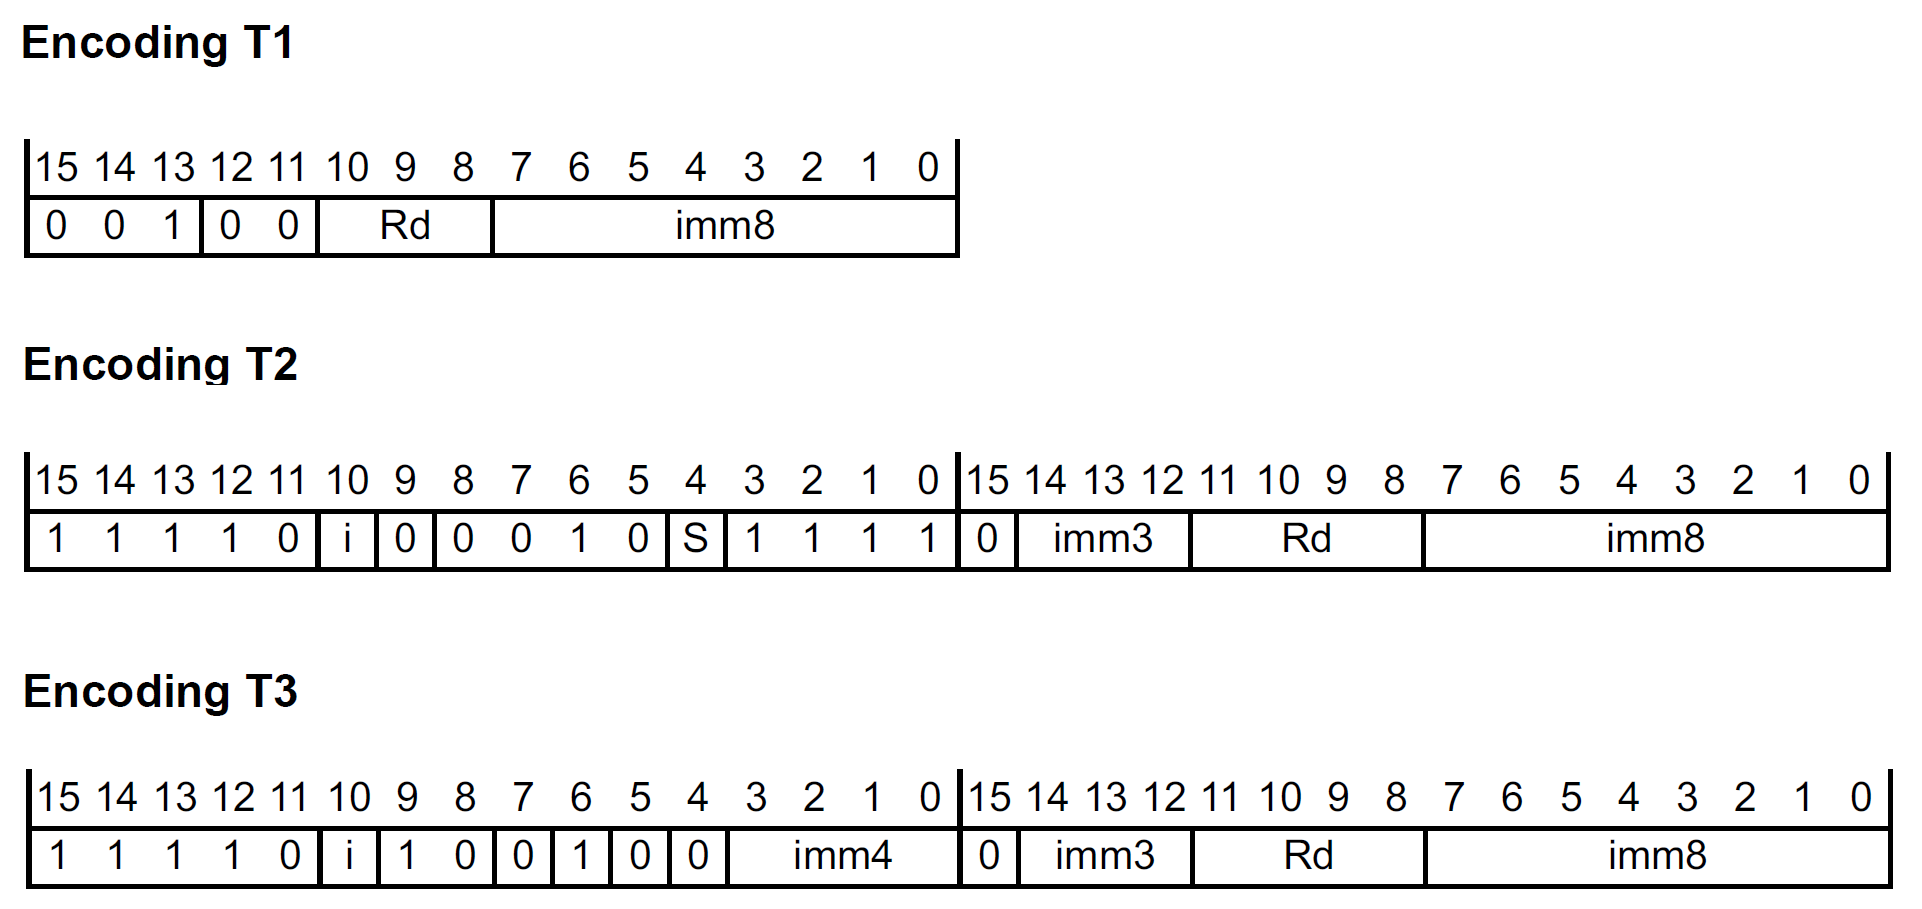
\includegraphics[scale=.32]{ch2-background/img/armv7-encoding.png}
                    \caption{Encodage de l'instruction MOV sur l'architecture ARMv7-M thumb2}
                    \label{fig:armv7-mov-encoding}
                \end{figure}
                
                \paragraph{}
                La modification des données consiste à changer les bits dans un registre du processeur, sur un bus mémoire pendant son transit ou dans la mémoire. La corruption de registre est également un modèle très étudié dans l'analyse au niveau binaire \cite{Blomer/CCS03, Verbauwhede/FDTC11}.
                De la même manière qu'au niveau matériel, différentes valeurs et plages de bits peuvent être considérées en fonction du  modèle de faute comme indiqué dans la figure \ref{tbl:bits}.
                Dans le domaine de la tolérance aux fautes, les modèles étudiés se restreignent souvent à une inversion de bit simple sur la donnée \cite{lu2015llfi, sharma2013towards, van2014evaluating, Georgakoudis/ICHPCNSA17, le2018resilience}. 
                Les modèles considérant la modification de plusieurs bits contiguës voire de fautes indépendantes existent \cite{CERN07}.
                La modification des données peut aussi correspondre à la modification d'une adresse ou de son calcul (comme un index de tableau par exemple).
                
                \paragraph{}
                Au niveau micro-architectural, c'est-à-dire en tirant parti des spécificités de l'architecture interne du processeur et des composants, des modifications plus subtiles peuvent être observées.
                Rivière et al. \cite{Riviere/HOST15} montrent qu'il est possible d'exploiter le tampon de pré-chargement du processeur (\textit{prefetch buffer}) pour annuler son remplissage et ainsi répéter une instruction en ignorant une partie des instructions suivantes.
                Le rejeu d'instruction \cite{Riviere/FPS14} consiste à exécuter deux fois une instruction, par exemple en attaquant la valeur du \gls{pc}, ou de la pipeline du processeur.
                Lorsqu'il s'accompagne du saut de l'instruction suivante, il peut s'assimiler à un remplacement de l'instruction.
                Plus récemment, Laurent et al. proposent des exploitations de fautes sur la micro-architecture, avec notamment des effets sur le processeur non-observables sur le jeu d'instructions \cite{Laurent/ECDSD19, Laurent/DATE19}.
                Par ailleurs, les modèles de faute visant les caches du processeur correspondent à des modèles ciblant la micro-architecture du processeur.
                
            \subsubsection{Modèle au niveau source}
            \label{sec:model:source}
            
                A plus haut niveau, les modèles de faute s'intéressent davantage aux modifications de la logique algorithmique du programme. En fonction de si on se place au niveau du code source ou d'un niveau intermédiaire, la granularité des fautes peut varier.
                La figure \ref{fig:software-models-scheme} présente une classification des modèles de faute au niveau source.
                Deux grandes classes de modèles de faute se dégagent de la littérature: l'\textit{altération des chemins d'exécution} du programme et la \textit{modification des données}. 
                
                \begin{figure}[ht!]\centering
                  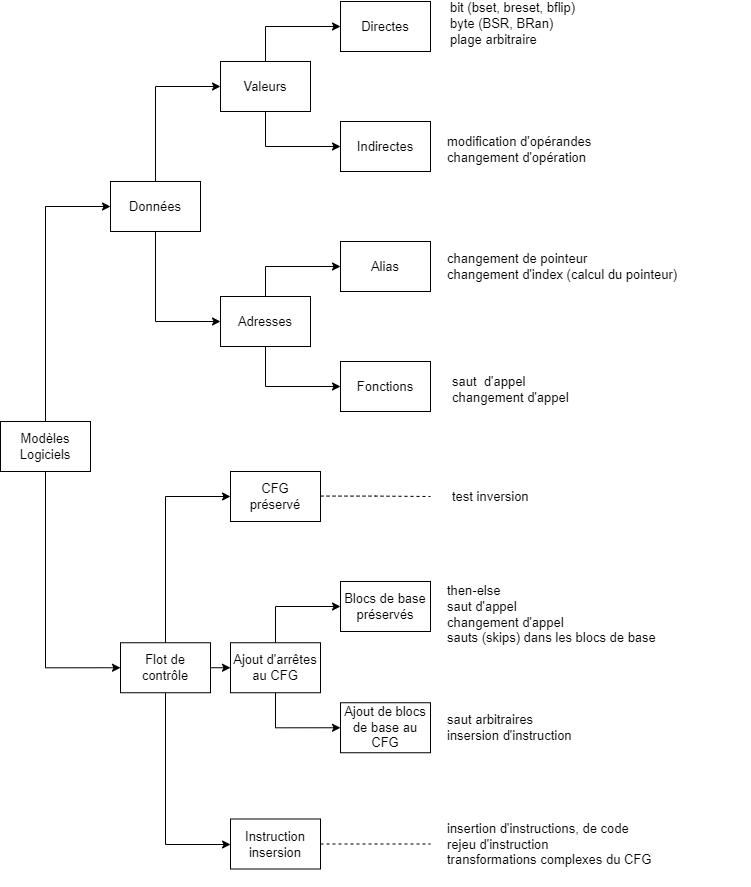
\includegraphics[scale=0.49]{ch2-background/img/Class Logiciel.drawio.png}
                  \caption{Classification des modèles de faute au niveau source}
                  \label{fig:software-models-scheme}
                \end{figure}
            
                L'altération des chemins d'exécution concerne les fautes ayant un effet sur l'intégrité du flot de contrôle \cite{Abadi/TISSEC09, Sayeed/AS19}. Il s'agit de détourner le flot d'exécution de son comportement normal.
                Le \textit{graphe de flot de contrôle} (\gls{cfg}) est une représentation du flot de contrôle du programme correspondant à un graphe orienté. 
                Les nœuds sont des blocs de base qui correspondent à une suite d'instructions atomiques (toujours exécutées en séquence).
                Les arêtes correspondent aux branchements conditionnels et aux sauts.
                Ainsi la figure \ref{fig:software-models-scheme} distingue les modèles axés sur la modification du flot de contrôle en fonction de leur impact sur le graphe de flot.
                
                Le modèle de l'inversion de test \cite{Berthome/ARES12, Potet/ICST14, Dureuil/PPLCC16} consiste à inverser le chemin sélectionné après une opération de branchement conditionnel. 
                Dans \cite{Bouffard/SCRAA11}, Bouffard et al. parviennent à modifier le flot de contrôle d'un programme Java Card\footnote{Plateforme Java minimaliste embarquée pour les cartes à puce.} en attaquant l'adresse de retour d'une fonction.
                Les modèles basés sur le saut d'instructions existent aussi au niveau source \cite{Moro/FDTC13, Potet/ICST14, Barry/CSCS16, Breier/TDSC19}.
                Ils ont généralement une granularité plus faible au niveau logiciel qu'au niveau matériel, comme par exemple dans \cite{lalande}, où Lalande et al. s'intéressent à un modèle de saut d'instructions au niveau du langage C. Il peut aussi s'agir de sauts d'appels de fonction \cite{Dureuil/PPLCC16}.
                Ces modèles attaquant l'intégrité du flot de contrôle sont un sujet important au niveau source, car ils induisent des comportements difficiles à anticiper et peuvent produire des nouveaux chemins dans l'application, que ce soit dans les outils d'analyse de robustesse tels que SmartCM \cite{Machemie/IFS11}, l'évaluation de contre-mesures \cite{Sere/IJSIA11} ou l'introduction de contre-mesures, par exemple à la compilation \cite{Werner/ICSCRAA15}. 
                
                La modification de données s'apparente principalement à la modification des valeurs lues ou écrites dans les variables, ou les valeurs temporaires utilisées pour calculer les expressions (i.e. les registres).
                Breier et al \cite{Breier/TDSC19} étudient l'effet d'un nombre arbitraire d'inversions de bits dans un registre. 
                La modification d'une donnée lors de la lecture en mémoire est également un modèle standard dans l'analyse de robustesse au niveau logiciel \cite{Moro/FDTC13, Berthome/ARES12}. 
                Le modèle d'inversion de bit dans une zone mémoire est aussi fréquemment utilisé dans le domaine de la tolérance aux fautes \cite{Benso/TODAES98, Georgakoudis/ICHPCNSA17}.
                L'attaque \textit{Rowhammer} \cite{Kim/ACM14} qui a été abordée dans le chapitre \ref{chpt:contexte} correspond à une modification de données sur la mémoire.
                
                \paragraph{}                
                La modification de données peut avoir un effet sur le flot de contrôle, par exemple dans le cas d'une faute d'une adresse de retour, d'une adresse de fonction, d'une adresse lors d'un saut arbitraire, et plus généralement lorsqu'une valeur est utilisée par la suite dans une condition ou un saut. 
                A l'inverse, le flot de contrôle peut avoir un effet comparable à une mutation de donnée puisque le flot détourné peut modifier des données différemment du comportement normal du programme.
                Lacombe et al \cite{lacombe2021combining} proposent un modèle visant les expressions au niveau CIL (représentation intermédiaire de l'outil Frama-C), permettant de considérer à la fois les modifications de données arbitraire et les fautes visant le flot de contrôle (avec la mutation de la valeur finale de l'expression dans les conditions). 
                
        \subsection{Classification des modèles au niveau logiciel}
        \label{sec:model-classification}
        
            Les sections précédentes ont présenté les problématiques liées à la mise en relation des modèles de faute à différents niveaux de représentation.
            Celles-ci concernent à la fois la représentativité des modèles étudiés à haut niveau par rapport à la réalité physique, la difficulté de l'observation et de la caractérisation des fautes et la compréhension de leurs effets \cite{Dureuil/CARDIS15, werner2020end}.
            Cette sous-section vise à présenter différentes approches pour classifier les modèles au niveau logiciel ainsi que la difficulté pour faire correspondre des modèles de niveaux différents.
            
            La figure \ref{fig:software-models-scheme} présentée dans la section \ref{sec:model:source} fait une première distinction entre les modèles sur le flot de contrôle et ceux sur les données. 
            La classification des modèles source peut aussi être réalisée en partant de la cible des fautes à bas niveau (instructions, données, registres, pipeline etc.).
            C'est en partie l'approche qui est utilisée dans la figure \ref{fig:arch-models-scheme} présentant les modèles au niveau architectural.
            La modification de données sur des zones différentes de l'architecture implique alors des modèles haut niveaux très variables.
    
            Une autre solution serait de classifier les modèles en fonction de l'inclusion de l'ensemble des fautes pouvant être réalisées. Cela peut être fait en considérant l'espace de faute de chaque modèle ou bien en comparant les comportements obtenus par chaque modèle. Il est par exemple possible de considérer qu'un modèle de mutation de donnée est un sous-ensemble d'un modèle de modification arbitraire de donnée ou encore qu'une inversion de test peut correspondre, en partie, à un cas spécifique du saut d'instruction lorsqu'on se place au niveau de représentation \gls{isa}.
            Cependant, cette approche a ses limites puisque les espaces de fautes de deux modèles peuvent ne pas avoir de relation d'inclusion et selon le niveau de représentation choisi, les relations entre les modèles de faute peuvent être très différentes. 
            La combinaison de modèles de faute et la prise en considération de fautes multiples compliquent encore cette notion d'inclusion\footnote{Par exemple, un modèle de mutation de donnée sur une instruction d'écriture de mémoire (store) peut être simulée par un nombre non borné de mutations de donnée en lecture (load).}.  
            
            Cela illustre la difficulté de faire correspondre des modèles à des niveaux de représentation différents et la question de la légitimité de raisonner à propos de modèles trop bas niveau lorsqu'on considère un programme au niveau logiciel.
            Les programmes doivent faire face à des attaquants très variés, et la définition ainsi que la modélisation des fautes sont des difficultés de l'évaluation de la robustesse d'un programme.
            Les modèles au niveau logiciel visent à être suffisamment génériques pour couvrir un maximum les modèles pouvant effectivement être observés mais sans viser la correspondance exacte avec ces modèles bas niveau et s'orientent plutôt vers la prise en compte de la logique algorithmique du programme. 
                    
    \section{Protection contre les attaques physiques}
    \label{sec:fi-protections}
        
        Afin de lutter contre les attaques physiques, de nombreuses solutions de protections ont été proposées \cite{BarEl/IEEE06, Yuce/HSS18}. 
        Ces protections peuvent prendre des formes variées en fonction du niveau de représentation et du modèle d'attaquant considéré. Cette section vise à donner un court aperçu des protections contre les attaques par injections de faute et les attaques physiques (fautes accidentelles et canaux auxiliaires). 
        Le chapitre \ref{chpt:placement} approfondit les problématiques liées à l'analyse et l'évaluation de protections dans le cadre d'attaques en fautes et présente un état de l'art des protections logicielles existantes dans la littérature.
        
        \begin{defi}
            Une \textit{protection} correspond à toute modification du programme, de l'architecture ou du matériel et de leurs fonctionnements visant à empêcher une attaque d'aboutir, la détecter, la corriger ou la rendre plus difficile à effectuer.
        \end{defi}
        
        \begin{defi}
            Une \textit{contre-mesure} est une protection visant à détecter une attaque afin de pouvoir ensuite la signaler, la corriger ou prendre des mesures comme le redémarrage du système ou sa coupure.
        \end{defi}
        
        Au niveau physique, les protections peuvent prendre la forme de détecteurs surveillant la tension d'alimentation ou la fréquence du circuit \cite{Zussa/DATE14}. 
        Les boucliers actifs (\textit{active shields}) \cite{BarEl/IEEE06} correspondent à un maillage métallique dans lequel les données circulent en continue. Si le maillage est endommagé ou modifié, le circuit ne fonctionne plus.
        Les détecteurs physiques permettent de réagir à une fréquence ou une tension inhabituelle \cite{BarEl/IEEE06}. 
        Les protections visant à limiter la connaissance de l'attaquant en rendant l'observation plus difficile sont très fréquentes dans le domaine des canaux auxiliaires. Parmi les protections physiques de ce type on peut citer le chiffrement de la mémoire \cite{Barenghi/IEEE2012} ainsi que l'ajout d'aléa dans la consommation de courant par exemple \cite{Moro/Phd14} ou encore dans l'ordonnancement des instructions \cite{Wittman/RSA08}.
        
        Au niveau architectural, la tâche de l'attaquant peut être rendue plus ardue en utilisant un encodage pour le jeu d'instructions compliquant attaques: par exemple un encodage différent de \texttt{0} pour l'instruction \gls{nop} est une solution pour se protéger contre les attaques de mise-à-0.
        Des protections par redondance des calculs ou des données peuvent par exemple être obtenues en ayant deux circuits de calcul dans le processeur ou l'\gls{alu}, qui comparent ainsi leur résultats, cette redondance pouvant être étendue à $n$ circuits redondants \cite{BarEl/IEEE06}.  
        
        Au niveau logiciel, les protections peuvent être appliquées sur toute la couche logicielle. On distinguera les protections appliquées en tant que transformation du programme et celles appliquées au niveau du système (système d'exploitation par exemple). 
        Les protections qui effectuent une transformation du programme source peuvent être appliquées à plusieurs niveaux de représentation du programme. 
        L'utilisation d'instructions idempotentes afin de se protéger contre les sauts d'instructions \cite{Moro/Phd14} a été proposée au niveau assembleur tandis que des protections ont été proposées au niveau du langage C \cite{lalande} ou lors de la compilation \cite{Barry/CSCS16, Proy/TACO17}. 
        Certaines approches visent la protection de l'intégrité du flot de contrôle par des mécanismes de signature de blocs ou de fonctions \cite{Oh/TR02, Reis/ISCCO05, Ferriere/LLVM19} ou encore par l'utilisation d'une \textit{pile cachée} \cite{Dureuil/CARDIS15} par exemple.
        L'utilisation de booléens endurcis visent à compliquer la tâche de l'attaquant d'une façon similaire à l'exemple de l'encodage du \gls{nop} pour le niveau architectural.
        
        Une partie des protections physiques, notamment celles basées sur la redondance des calculs ou de la mémoire, ou le chiffrement de celle-ci, peuvent être implémentées à plus haut niveau. Cependant, les protections logicielles peuvent être limitées par rapport à leurs équivalents physiques. En général, les systèmes sont protégés en combinant différents niveaux de protection \cite{Yuce/HASSP16}.
        
        \begin{figure}[htb]\centering
          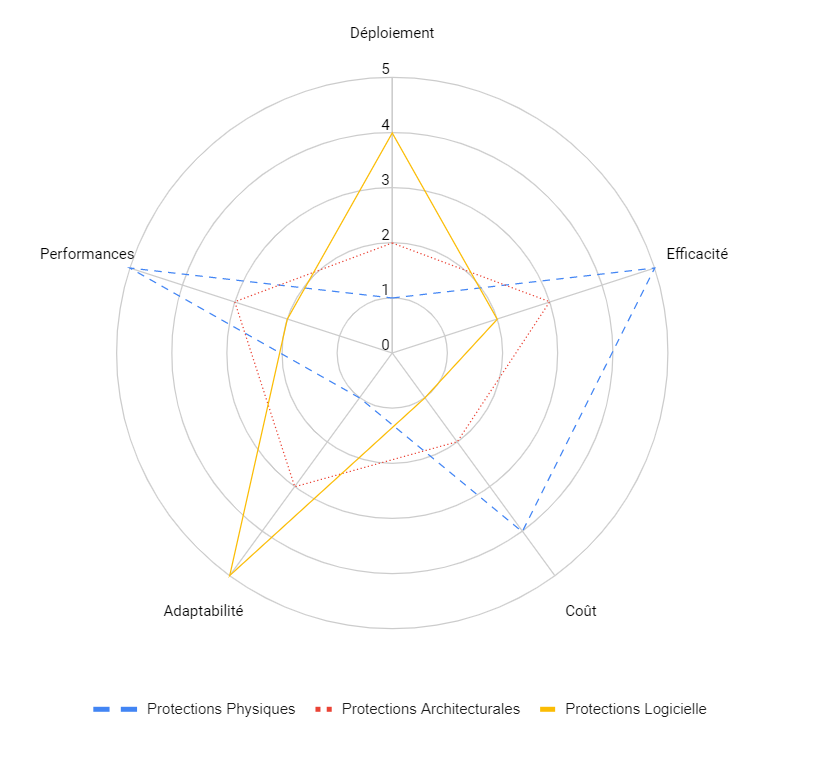
\includegraphics[scale=.58]{ch2-background/img/ch2-protections-caracs.png}
          \caption{Caractéristiques des protections à différents niveaux}
          \label{fig:ch2-protections}
        \end{figure}
        
        \paragraph{} La figure \ref{fig:ch2-protections} compare certaines caractéristiques des protections en fonction du niveau auquel elles sont introduites: 
        \begin{itemize}
            \item \textit{Portabilité}: capacité à s'adapter à une architecture ou une application donnée.
            \item \textit{Déploiement}: facilité de mise-à-jour de la protection.
            \item \textit{Efficacité}: capacité à protéger.
            \item \textit{Coûts}: coûts de développement et de mise en place.
            \item \textit{Performance}: taille du code, consommation mémoire et temps d'exécution ajoutés.
        \end{itemize}         
        
        Les protections physiques permettent de protéger l'ensemble des programmes d'un composant mais sont plus coûteuses à mettre en place et ne peuvent pas être modifiées une fois que le produit est déployé (une carte à puce par exemple). 	\`A l'inverse, les protections logicielles peuvent être ajoutées à l'aide de mises-à-jour logicielles. 
        Les protections de plus haut niveau peuvent ainsi être adaptées aux protections disponibles à plus bas niveau sur lesquelles elles peuvent s'appuyer.  
        Les protections bas niveau peuvent protéger des modules du système qui ne sont pas accessibles au niveau logiciel, mais ne peuvent pas être adaptées à un programme ou une pile logicielle particulière et visent une protection générique du composant.
        
        La protection contre les attaques en fautes est fortement compliquée contre les attaques en \textit{fautes multiples}.
     
    \section{Les fautes multiples}
    \label{sec:multi-fault}
        
        La littérature récente contient des exemples d'attaques en fautes multiples \cite{kim2007fault, Barenghi/IEEE2012, Natella/ACM16, SSTIC20}.
        
        Les fautes multiples rendent le processus de développement d'un programme sécurisé d'autant plus difficile que le nombre de configurations de fautes possibles sur un programme croît rapidement. Cette explosion combinatoire complique l'expertise humaine et l'analyse des outils pour l'évaluation de robustesse.
        De plus, la combinaison de plusieurs modèles de faute doit être considérée et rend plus complexe la protection et l'analyse de robustesse.
        
        Dans le cas de la protection d'un système, la présence de fautes multiples complique également la tâche. En effet, si plusieurs fautes peuvent être injectées, alors une protection peut elle-même être visée par une première faute pour rendre possible la seconde. Dans la fonction \textit{compare} du programme \texttt{verify\_pin} présentée dans le listing \ref{lst:verifyPIN-BAC-LC}, une première injection peut éviter la boucle \texttt{for} (par exemple avec une inversion de la condition \texttt{i < size}) et une seconde peut inverser la condition \texttt{if(i != size) killcard()} afin d'éviter la contre-mesure.
            
            
\lstset{caption={Compteur de boucle sur la fonction \texttt{compare}},label=lst:verifyPIN-BAC-LC}
\begin{lstlisting}     
bool compare(uint8_t* a1, uint8_t* a2, size_t size)
{
    bool result = true;
    for(size_t i = 0; i < size; ++i)
        if(a1[i] != a2[i])
            result = false;
    
    if(i != size) // Protection
        killcard();
        
    return result;
}
\end{lstlisting}
    
        Cette possibilité d'attaquer les protections elles-mêmes, d'autant qu'une grande partie de la littérature propose des contre-mesures visant principalement des fautes uniques, rend l'évaluation et la conception de protections plus complexes dans le contexte des fautes multiples.
        La prise en compte des fautes multiples pour l'analyse de robustesse de programme et pour l'analyse de protections est une problématique à laquelle cette thèse vise à répondre sur deux aspects:
        
        \begin{itemize}
            \item Maîtriser l'exploration des exécutions en multi-fautes malgré l'explosion combinatoire des chemins (chapitres \ref{chpt:lazart} et \ref{chpt:lazart-implem}).
            \item Aider à l'analyse et au placement des contre-mesures dans un contexte multi-fautes (chapitres \ref{chpt:placement} et \ref{chpt:ccpo}).
        \end{itemize}
        
        Avant de s'intéresser à l'outil Lazart, la suite de se chapitre se termine par une analyse des outils existants.
            
        \section[État de l'art des outils d'analyse de robustesse]{État de l'art des outils d'analyse de robustesse pour l'injection de faute}
    \label{sec:soa-tools}

        Cette section propose un aperçu des outils existants pour l'évaluation de robustesse dans le cadre de la tolérance aux fautes et des attaques par injection de fautes. Elle vise aussi à proposer un ensemble de critères pour la comparaison de ces outils. L'état de l'art des outils et des techniques d'analyse pour l'injection de fautes a déjà fait l'objet de plusieurs articles de recherche \cite{kooli2014survey, Given/ICESS17, gangolli2022systematic} et de surveys \cite{Christofi/Phd13, Dureuil/Phd16, Heydemann/HDR17}. Les outils visant la tolérance aux fautes sont également considérés.        
        
        \begin{figure}[ht]\centering
          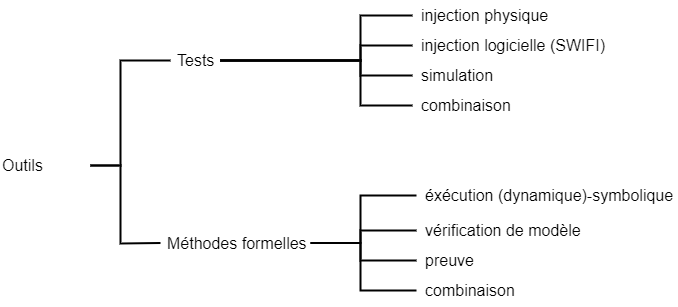
\includegraphics[scale=.45]{ch2-background/img/plan-soa-tools.drawio.png}
          \caption{Organisation et périmètre de l'état de l'art}
          \label{fig:soa-tools-scheme}
        \end{figure}
         
        La suite de cette section s'organise comme suit. La sous-section \ref{sec:soa-tools-carac} présente différents critères qui seront considérés pour la comparaison des outils. L'état de l'art est organisé en fonction de la technique d'analyse employée comme montré dans la figure \ref{fig:soa-tools-scheme}. Les sous-sections \ref{sec:soa-tools-test} et \ref{sec:soa-tools-formal} présentent respectivement les méthodes basées sur les tests et celles reposant sur les méthodes formelles.
        Enfin, la sous-section \ref{sec:soa-tools-conclusion} conclut cette section.
        
        \subsection{Caractéristiques des outils}
        \label{sec:soa-tools-carac}
     
            Différentes caractéristiques peuvent être considérées lorsqu'on s'intéresse à un outil d'analyse concernant les attaques en fautes.
            La figure \ref{fig:soa-tools-conclusion} présente une classification d'un ensemble de caractéristiques issus de la littérature et qui seront considéré dans cette section :
            
            \begin{figure}[hbt]\centering
              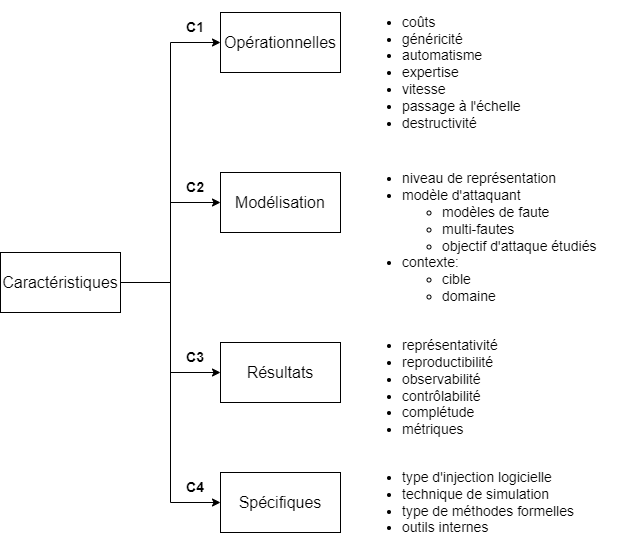
\includegraphics[scale=.55]{ch2-background/img/tools-carac.drawio.png}
              \caption{Classification des caractéristiques pour les outils d'analyse de robustesse contre les fautes}
              \label{fig:soa-tools-conclusion}
            \end{figure}
            
            \begin{itemize}
                \item[$\bullet$] \textbf{C1} Caractéristiques opérationnelles:
                \begin{itemize}
                    \item[-] \textit{Coûts}: regroupe les coûts liés au développement de l'outil en termes de moyens humains et de matériel ainsi que le niveau d'expertise requis par l'utilisateur pour l'utilisation de l'outil. 
                    \item[-] \textit{Généricité}: détermine à quel point l'outil est spécifique à un matériel ou une architecture donnée (on parlera à l'opposé de \textit{spécificité}).
                    \item[-] \textit{Automatisation}: niveau d'intervention de l'utilisateur requis.
                    \item[-] \textit{Expertise}: niveau d'expertise de l'utilisateur dans le domaine étudié ou la méthode d'analyse utilisée par l'outil. 
                    \item[-] \textit{Vitesse}:  comprend la vitesse d'exécution de l'outil pour une analyse ou encore le temps de mise en place nécessaire entre deux expérimentations. 
                    \item[-] \textit{Passage à l'échelle}: capacité de l'outil à analyser des programmes / systèmes complexes.
                    \item[-] \textit{Destructivité}: possibilité d'endommager le système étudié par l'analyse.
                \end{itemize}
                
                \item[$\bullet$] \textbf{C2} Caractéristiques liées à la modélisation:
                \begin{itemize}
                    \item[-] \textit{Niveau de représentation}: niveau de représentation de l'analyse (à ne pas confondre avec le niveau d'implémentation de l'outil).
                    \item[-] \textit{Modèle d'attaque}: modèles de faute supportés, support des fautes multiples et objectifs d'attaque étudiés.
                    \item[-] \textit{Contexte d'analyse}: 
                    \begin{itemize}
                        \item[$\circ$] \textit{Cible de l'analyse}: le type de système visé par l'analyse (programme, application, circuit, machines distribuées...).
                        \item[$\circ$] \textit{Domaine}: attaques en fautes, canaux auxiliaires ou fautes accidentelles.
                    \end{itemize}
                \end{itemize}                
                
                \item[$\bullet$]\textbf{C3} Caractéristiques liées aux résultats:
                \begin{itemize}
                    \item[-] \textit{Représentativité}: représentativité des résultats obtenus par rapport à une véritable attaque. 
                    \item[-] \textit{Reproductibilité}: détermine si les résultats obtenus peuvent facilement être reproduits. 
                    \item[-] \textit{Observabilité}: correspond à la capacité de la méthode d'observer l'effet des fautes injectées. 
                    \item[-] \textit{Contrôlabilité}: détermine le contrôle qu'offre la méthode sur les fautes qui seront injectées.
                    \item[-] \textit{Complétude}: couverture des exécutions fautées par l'analyse.
                    \item[-] \textit{Métriques}: métriques produites par l'outil.
                \end{itemize}
                
                \item[$\bullet$]\textbf{C4} Caractéristiques spécifiques: sous-classe de la technique d'analyse, technique d'implémentation.
            \end{itemize}
            
            Les caractéristiques suivantes, correspondant à des combinaisons de caractéristiques, seront aussi étudiées :
            \begin{itemize}
                \item \textit{Performance} (\textbf{C1}): passage à l'échelle et vitesse.
                \item \textit{Mise-en-place} (\textbf{C1}): regroupe les coûts lié au développement de l'outil en termes de moyens humains et de matériel et la destructivité.
                \item \textit{Accessibilité} (\textbf{C1}\&\textbf{C3}): regroupe les caractéristiques de l'expertise requise pour l'utilisateur, l'automatisme et la contrôlabilité.
            \end{itemize}
            
        \subsection{Outils basés sur le test}
        \label{sec:soa-tools-test}
        
            Cette sous-section s'intéresse aux outils basés sur le test, c'est-à-dire qui effectuent une sous-approximation des exécutions.
            Cette classe regroupe un grand nombre de techniques et d'outils:
            \begin{itemize}
                \item L'\textit{injection physique} (section \ref{sec:soa-tools-physic}) qui correspond à l'expérimentation en attaquant physiquement le système.
                \item L'\textit{injection logicielle} (section \ref{sec:soa-tools-swifi}) qui englobe tous les outils émulant l'effet des fautes physiques au niveau logiciel.
                \item La \textit{simulation}\footnote{Une partie de la littérature utilise le terme \textit{simulation} par opposition aux méthodes formelles \cite{kooli2014survey, Heydemann/HDR17}. Dans la suite de ce manuscrit, le mot \textit{simulation} ne sera pas employé en ce sens, parlant à la place d'\textit{outils basés sur les tests}.} (section \ref{sec:soa-tools-simu}) qui correspond aux outils exécutant le programme dans un simulateur dans lequel les fautes sont injectées.
            \end{itemize}        
        
            \subsubsection{Injection physique}
            \label{sec:soa-tools-physic}
            
                Une méthode d'injection de fautes physique (laser, glitches...) permet d'étudier le comportement du système soumis à des fautes. 
                Le terme \textit{injection de faute} a d'ailleurs émergé dans la littérature avant l'apparition des attaques par injection de fautes pour désigner des plateformes telles que MESSALINE \cite{Arlat/TSE90} ou encore RIFLE \cite{Madeira/DCC94}.
                Toute technique d'attaque par faute peut théoriquement être utilisée comme protocole de test physique pour un circuit.  
                
                \begin{figure}[hbt]\centering
                  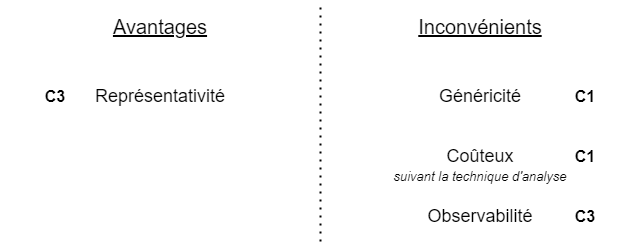
\includegraphics[scale=.45]{ch2-background/img/advantages-physics.drawio.png}
                  \caption{Caractéristiques de l'injection physique}
                  \label{fig:soa-tools-scheme-physic}
                \end{figure}
                
                La figure \ref{fig:soa-tools-scheme-physic} résume les avantages et inconvénients de ce type de techniques d'analyse. 
                L'indication $CI$ fait référence aux classes de caractéristiques présentées précédemment.
                L'injection physique à l'avantage d'obtenir des résultats très représentatifs sur la robustesse du programme puisque la faute est injectée directement sur le système à analyser et n'inclut donc pas d'étape intermédiaire ou d'abstraction pouvant fausser les résultats.
                L'observation et la caractérisation de la propagation des fautes observées sont difficiles et la mise en place d'un système d'observation peut introduire une perte de précision \cite{Faurax/Phd09, kooli2014survey}.
                
                La mise en place de tels bancs de test peut s'avérer coûteuse en fonction de la technique d'injection de fautes utilisée.
                Ces méthodologies d'analyse par injection physique sont souvent très spécifiques au système étudié par rapport à des approches plus haut niveau.
                De plus, certaines techniques d'injections destructrices peuvent endommager l'appareil étudié.
                Cependant, ces méthodes d'injections physiques sont utilisées pour la certification des composants sécurisés afin de démontrer la faisabilité d'une attaque.               
            
            \subsubsection{Injection au niveau logiciel (SWIFI)}
            \label{sec:soa-tools-swifi}
            
                Une autre technique très largement utilisée est la reproduction au niveau logiciel des fautes, ou de l'effet causé par des fautes au niveau de représentation considéré. 
                Cette technique désignée \gls{swifi} a émergé dès la fin des années 1980 \cite{Segall/FTCS88, Kanawati/FTCS92, Kao/TSE93} dans le milieu des fautes accidentelles pour ensuite se développer dans le domaine des attaques par injection de fautes jusqu'à aujourd'hui \cite{Georgakoudis/ICHPCNSA17}. 
                
                \paragraph{}         
                \gls{fiat} \cite{Segall/FTCS88} est l'un des premiers outils de type \gls{swifi} et a été proposé en 1988. Il vise l'analyse de systèmes distribués.
                Les fautes autorisées sont décrites par l'utilisateur à l'aide d'un langage spécifique et sont ensuite générées lors de la campagne d'expérimentation. Cet outil a notamment été utilisé pour analyser des fautes de type mise-à-zéro et mise-à-un d'octets et l'inversion de deux bits complémentaires \footnote{C'est-à-dire deux bits de valeurs différentes, afin d'éviter d'être détecté par un code correcteur d'erreur simple.} \cite{Barton/TC90}.   
                \gls{fine} \cite{Kao/TSE93}, est une plateforme d'analyse qui considère à la fois les fautes physiques et les fautes liées à des erreurs d'implémentation ou de conception logicielle, et qui vise à étudier la propagation des fautes dans un système d'exploitation.
                L'outil injecte les fautes au niveau logiciel à l'aide d'un noyau UNIX modifié traçant l'exécution et proposant des appels systèmes supplémentaires.
                Les fautes matérielles consistent en une mutation de données dans la mémoire, les registres ou les bus. 
                Les fautes logicielles sont implémentées en tant que modifications du programme binaire et incluent: données mal initialisées, assignation incorrectes, vérifications des cas d'erreurs incomplètes ou encore mauvaise sortie du programme.
                L'outil vise aussi à étudier comment les erreurs se propagent entre les différentes machines et les différents niveaux.
    
                L'outil \gls{define} \cite{Kao/FTPDS94} est une évolution de \gls{fine} qui supporte l'injection dans un système distribué. Celui-ci permet l'injection dans chaque machine, dans n'importe quelle application en mode utilisateur ou superviseur. 
                En plus des appels systèmes rajoutés et de la modification de l'image binaire du programme déjà utilisées dans \gls{fine}, \gls{define} utilise un handler modifié d'interruptions de l'horloge matérielle afin de contrôler l'injection des fautes dans les bus et la mémoire.
                Des expérimentations ont été menées sur un ensemble de 7 machines SunOS pouvant être fautées, l'une d'entre elles étant utilisée comme serveur. Les auteurs constatent que les erreurs sur le serveur se révèlent plus critiques en général que les fautes sur le client. 
                
                \gls{exfi} \cite{Benso/TODAES98} est un environnement d'injection de fautes qui utilise le \textit{trap execution mode} des microprocesseurs pour l'injection de fautes.
                Ainsi, \gls{exfi} ne nécessite pas de matériel spécialisé (comme FERRARI \cite{Kanawati/FTCS92} par exemple) ou la présence d'un système d'exploitation (comme les outils utilisant des traps logicielles type \gls{fine}).
                Une passe est utilisée pour réduire cet ensemble de fautes en fonction de règles spécifiques permettant d'écarter certaines fautes sans perdre en précision. 
                Ces règles visent à écarter les fautes qui n'auraient pas d'effet sur le système, seraient forcément détectées par un mécanisme de détection d'erreur et celles dont le comportement est déjà couvert par une autre faute de la liste.
                \gls{exfi} supporte un modèle de fautes temporaires de type bit-flip pouvant cibler les instructions, la mémoire et les registres.
                Une faute est caractérisée par le nombre d'instructions depuis le démarrage de l'application.
                
                \gls{llfi} \cite{Thomas/SELSE13, Lu/SQRS15}, proposé en 2013, est un outil pour la tolérance aux fautes travaillant sur la représentation intermédiaire \gls{llvm}.
                Celui-ci instrumente le programme à analyser et génère un exécutable pour l'injection de fautes et un exécutable de profilage déterminant quelles fautes vont être injectées.
                \gls{llfi} modélise des inversions de un ou deux bits et vise une douzaine d'instruction comprenant le calcul d'adresse (\texttt{load} et \texttt{store}) ou encore les opérations arithmétiques (\texttt{mul}, \texttt{fmul} etc.).
                L'outil ne considère que les fautes \textit{activées}, c'est-à-dire lorsque la donnée fautée est lue par le programme avant d'être écrasée par une autre instruction.
                Les auteurs constatent sur leurs expérimentations que certaines instructions (comme les instructions de comparaison)
                sont moins sensibles aux fautes que d'autres et que deux inversions augmentent le risque de crash sans augmenter le nombre d'erreurs de calcul non détectées.
    
                REFINE \cite{Georgakoudis/ICHPCNSA17} est une approche basée sur l'injection de fautes à la compilation qui vise à modéliser plus finement des comportements qui sont difficiles à capter au niveau d'une représentation intermédiaire (comme par exemple les prologues / épilogues de fonctions qui sont abstraits par l'IR LLVM).
                REFINE se situe dans le backend du compilateur et a ainsi accès aux instructions spécifiques (au prix de la portabilité).
                L'outil se place ainsi après toutes les passes d'optimisation afin d'éviter que le code injecté puisse être transformé par le compilateur. 
                REFINE se concentre sur un modèle de mutation d'opcode et d'opérande, ignorant les opcodes invalides.
                Les auteurs comparent leur approche à celle de \gls{llfi} qui s'applique également au niveau de l'IR \gls{llvm} et PINFI (qu'ils ont modifiés) qui travaille au niveau binaire sur différents programmes de calcul haute performance (\gls{hpc}).
                Ils indiquent que les performances et la précision de REFINE sont meilleures que celles de \gls{llfi} et égalent, voire dépassent dans certains cas, celles de PINFI. 
            
                \centerline{}
                \begin{table}[hbt]
                    {\tiny
                    \begin{center} 
                    \setlength\tabcolsep{4pt}
                    \begin{tabular}{|l|l|c|c|c|c|c|c|}
                    \hline
                    \multicolumn{1}{|c|}{Outil} & \multicolumn{1}{c|}{Niveau} & Technique & Modèle & Fautes & Cible & Oracle & FI \\ \hline
                    \begin{tabular}[c]{@{}l@{}}FIAT \\ \cite{Segall/FTCS88}\end{tabular} & Physique & \begin{tabular}[c]{@{}c@{}}materiel, OS\\ spécialisé\end{tabular} & \begin{tabular}[c]{@{}c@{}}mémoire\\ registres\\ communication\end{tabular} & 1 & \begin{tabular}[c]{@{}c@{}}système\\ distribué\end{tabular} & SDC & Non \\ \hline
                    \begin{tabular}[c]{@{}l@{}}Ferrari \\ \cite{Kanawati/FTCS92}\end{tabular} & Physique & \begin{tabular}[c]{@{}c@{}}software-trap\\ (syscall)\\ materiel spécialisé\end{tabular} & \begin{tabular}[c]{@{}c@{}}mémoire, registre\\ remplacement inst.\\ fautes permanentes\end{tabular} & 1 & \begin{tabular}[c]{@{}c@{}}système\\ distribué\end{tabular} & SDC & Non \\ \hline
                    \begin{tabular}[c]{@{}l@{}}DEFINE \\ \cite{Kao/FTPDS94}\end{tabular} & UNIX & \begin{tabular}[c]{@{}c@{}}kernel modifié\\ interrupt modifiées\end{tabular} & \begin{tabular}[c]{@{}c@{}}CPU (ALU, cache,\\ decoder, reg, bus), \\ communication\\ fautes de design\end{tabular} & 1 & \begin{tabular}[c]{@{}c@{}}système\\ distribué\end{tabular} & SDC & Non \\ \hline
                    \begin{tabular}[c]{@{}l@{}}Xception \\ \cite{Carreira/IEEE98}\end{tabular} & CPU & \begin{tabular}[c]{@{}c@{}}fonctionnalité\\ CPU\end{tabular} & \begin{tabular}[c]{@{}c@{}}flips, sa1, sa0, bit mask\\ CPU registre bus\end{tabular} & 1 & application & SDC & Non \\ \hline
                    \begin{tabular}[c]{@{}l@{}}EXFI \\ \cite{Benso/TODAES98}\end{tabular} & µkernel & software-trap & \begin{tabular}[c]{@{}c@{}}bitflip\\ (mem / reg)\end{tabular} & 1 & application & SDC & Non \\ \hline
                    \begin{tabular}[c]{@{}l@{}}LLFI \\ \cite{Thomas/SELSE13}\end{tabular} & LLVM & compilation & \begin{tabular}[c]{@{}c@{}}flip ALU\\ store / load\end{tabular} & 1 & application & SDC & Non \\ \hline
                    \begin{tabular}[c]{@{}l@{}}REFINE \\ \cite{Georgakoudis/ICHPCNSA17}\end{tabular} & LLVM & compilation & \multicolumn{1}{l|}{bit-flip sur opérandes} & 1 & \multicolumn{1}{l|}{\begin{tabular}[c]{@{}l@{}}application\\ (HPC)\end{tabular}} & SE & Non \\ \hline
                    \end{tabular}
                \end{center}
                }       
                \caption{Comparaison de quelques outils de type SWIFI \label{tbl:tools-swifi}}
                \end{table}

                \paragraph{}
                La table \ref{tbl:tools-swifi} présente une comparaison de quelques outils de type \gls{swifi}.
                La colonne \textit{Niveau} indique le niveau d'abstraction auquel se place l'outil.
                La colonne \textit{Technique} correspond à la méthode utilisée pour émuler les fautes au niveau logiciel.
                La colonne \textit{Modèle} précise les modèles de faute supportés et la colonne \textit{Faute} la limite de faute pour les attaques.
                La colonne \textit{Cible} correspond au type de système étudié par l'outil (système distribué, application etc.).
                La colonne \textit{Oracle} indique le type de propriété de sécurité ou de sûreté étudiée par l'outil. Ici \textit{SDC} fait référence aux corruptions silencieuses de données.
                Enfin, la colonne \textit{FI} détermine si l'outil vise le milieu des attaques par injection de fautes ou celui des fautes accidentelles (ici tous).
                
                La figure \ref{fig:soa-tools-scheme-swifi} résume les avantages et inconvénients des outils \gls{swifi} comparés aux méthodes d'injection physiques. L'injection logicielle est généralement moins coûteuse, plus facile à mettre en place et plus générique.
                L'observabilité est également supérieure avec les approches d'injection logicielle, qui peuvent tirer partie de certaines technologies comme les exceptions matérielle (\gls{exfi}) \cite{Benso/TODAES98}.
                
                \begin{figure}[htpb]\centering
                  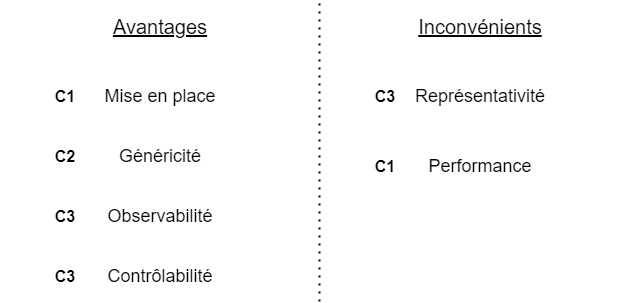
\includegraphics[scale=.41]{ch2-background/img/advantages-swifi.drawio.png}
                  \caption{Caractéristiques des méthodes SWIFI comparées à l'injection physique}
                  \label{fig:soa-tools-scheme-swifi}
                \end{figure}
                
                La sur-couche logicielle pour émuler la faute offre une représentativité moindre par rapport à l'injection physique et peut aussi ajouter une surcharge qui diminue les performances. Cette perte de précision dépend de la technique d'injection logicielle utilisée et des optimisations ont été développées qu'il s'agisse de représentativité ou de performance \cite{Lu/SQRS15, Georgakoudis/ICHPCNSA17}.
    
            \subsubsection{Outils basés sur la simulation}
            \label{sec:soa-tools-simu}
            
                La simulation désigne les outils qui effectuent une exécution sur un système simulé, sans exécuter directement sur le matériel étudié. 
                Les caractéristiques de l'outil dépendent alors en grande partie de la modélisation du système dans le simulateur.
                
                \paragraph{} 
                Depend \cite{Goswami/TC97} est un simulateur qui vise à prendre en compte les interactions entre les différents composants d'un système complexe en cas de fautes accidentelles.
                L'outil modélise le système en C++ afin de simuler des fautes au niveau des portes logiques. 
                Depend est capable de simuler des fautes sur la mémoire (bit-flip) et dans les communications (paquet perdu, corruption...). Les fautes sont décrites par l'utilisateur en C++ également.
                
                SINJECT \cite{Zarandi/DFTVS03} est un outil qui analyse la robustesse face aux fautes accidentelles au niveau de la représentation \gls{vhdl} et Verilog. 
                Il permet d'injecter un large nombre de fautes physiques au niveau des données et du circuit. Ceux-ci sont introduits dans le système Verilog à partir d'une description utilisateur. L'injection en \gls{vhdl} est faite avec la technique mutant-saboteurs.
                L'outil profite du mode combiné \gls{vhdl}/Verilog permettant de profiter de la représentativité de Verilog et de la description \gls{vhdl}.
                SINJECT s'intéresse à des objectifs d'attaque de tolérance aux fautes sur les traces simulées.
                
                \gls{pafi} \cite{Faurax/CSS06, Faurax/Phd09} est un outil étudiant les fautes au niveau du circuit utilisant la modélisation Verilog et \gls{vhdl}. 
                Il vise à vérifier l'absence de fuite de données secrètes dans le cadre d'attaques en multi-fautes au niveau circuit.
                L'outil s'appuie sur le simulateur Cadence NCSim (un outil propriétaire de STMicroelectronics) et utilise le fichier de commandes du simulateur pour contrôler les fautes à injecter.
                Une pondération basée sur des critères définis en fonction du modèle de faute permet de sélectionner les fautes à simuler (bit-flip sur les bascules ou faute sur les délais dans le circuit), ce qui permet un meilleur passage à l'échelle en multi-fautes.
                Par ailleurs, l'outil prend en compte les mécanismes de détection et indique les faux-positifs, faux-négatifs, attaques non détectées et attaques détectées.
                L'outil se veut extensible et générique en proposant un moyen de définir le modèle de circuit et les modèles de faute.
                
                \begin{sloppypar}   
                Celtic \cite{Dureuil/Phd16, Werner/Phd22} est un simulateur au niveau binaire développé en C++ qui permet de simuler des fautes au niveau de l'\gls{isa} et de l'architecture.
                Celtic supporte les fautes comme le saut d'instruction, la corruption du cache d'instruction \cite{Riviere/HOST15} et les attaques sur les données sur les registres, la mémoire et le décodage des instructions. L'outil supporte également les fautes multiples, ceci étant facilité par la parallélisation des simulations.
                L'objectif d'attaque est exprimé dans le programme et évalué pour chaque trace simulée afin de récupérer les attaques réussies.
                Celtic propose un langage de spécification d'architecture (GISL) permettant d'adapter facilement l'outil à différentes architectures. 
                \end{sloppypar}   
            
                \begin{table}[h]
                {\tiny
                \begin{center}                
                \setlength\tabcolsep{3.9pt}
                    \begin{tabular}{|l|l|l|l|l|l|l|l|l|}
                    \hline
                    Outil & Niveau & Implem & Simu type & Modèle & Fautes & Cible & Oracle & FI \\ \hline
                    FOCUS \cite{Choi/TC92} & Physique & VLSI & externe & porte logiques & X & \begin{tabular}[c]{@{}l@{}}systèmes\\ distribués\end{tabular} & SDC & Non \\ \hline
                    Depend \cite{Goswami/TC97} & \begin{tabular}[c]{@{}l@{}}Circuit\\ µ-arch\end{tabular} & C++ & intégrée & \begin{tabular}[c]{@{}l@{}}circuit\\ communication\\ mem.\end{tabular} & 1 & \begin{tabular}[c]{@{}l@{}}systèmes\\ distribués\end{tabular} & SDC & Non \\ \hline
                    SINJECT \cite{Zarandi/DFTVS03} & \begin{tabular}[c]{@{}l@{}}Verilog /\\ VHDL\end{tabular} & \begin{tabular}[c]{@{}l@{}}Verilog /\\ VHDL\end{tabular} & intégrée & circuit & 1 & application & SDC & Non \\ \hline
                    PAFI  \cite{Faurax/CSS06} & Circuit & \begin{tabular}[c]{@{}l@{}}Verilog /\\ VHDL\end{tabular} & externe & \begin{tabular}[c]{@{}l@{}}bit-flip\\ délais\end{tabular} & X & \begin{tabular}[c]{@{}l@{}}Verilog /\\ VHDL\end{tabular} & \begin{tabular}[c]{@{}l@{}}SC\\ exploit-\\ abilité\\ blocage\end{tabular} & Oui \\ \hline
                    CELTIC  \cite{Werner/Phd22} & x86 & C++ & intégrée & \begin{tabular}[c]{@{}l@{}}data (reg, mem)\\ cache, saut, rejeu\end{tabular} & X & x86 & \begin{tabular}[c]{@{}l@{}}oracle\\ logiciel\end{tabular} & Oui \\ \hline
                    \end{tabular} \end{center}
                }            
                \caption{Comparaison de quelques outils de simulation \label{tbl:tools-simu}}
                \end{table}

                La table \ref{tbl:tools-simu} présente une comparaison de plusieurs outils de simulation.
                Les colonnes \textit{Niveau}, \textit{Modèle}, \textit{Cible}, \textit{Oracle} et \textit{FI} ont la même signification que pour la table des outils \gls{swifi}. 
                La colonne \textit{Fautes} indique la limite de faute, le symbole "X" indiquant le support des fautes multiples.
                La colonne \textit{Implem} correspond au niveau auquel l'outil est implémenté (ce qui peut être différent du niveau de représentation étudié par l'outil).
                La colonne \textit{Simu type} indique si l'injection de fautes est intégrée au simulateur ou si les fautes sont émulées pour un simulateur existant.
                
                La figure \ref{fig:soa-tools-scheme-simu} présente les avantages et inconvénients de la simulation par rapport aux méthodes d'analyse présentées précédemment.
                En fonction de la modélisation du système par le simulateur, la généricité de l'outil et la représentativité des résultats peuvent être très variables. La généricité de l'approche est en relation directe avec le niveau de représentation du simulateur mais dépend aussi des choix du simulateur, GISL permettant par exemple une portabilité d'architecture pour CELTIC.
                Le développement d'un simulateur pour un système donné est le plus généralement coûteux par rapport à l'injection logicielle, mais le simulateur peut être disponible avant le matériel simulé ce qui a un intérêt dans le cycle de développement. 
                Les performances sont souvent moins bonnes qu'avec les approches citées précédemment.
    
                \begin{figure}[hbt]\centering
                  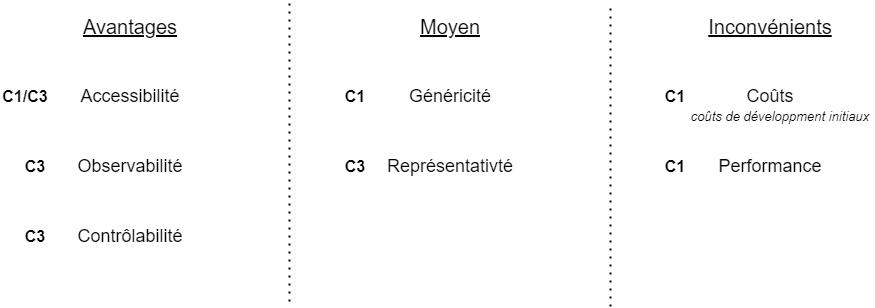
\includegraphics[scale=.56]{ch2-background/img/advantages-simu.drawio.png}
                  \caption{Comparaison des outils de simulation par rapport aux méthodes précédentes}
                  \label{fig:soa-tools-scheme-simu}
                \end{figure}
                
                On peut également opposer les simulateurs qui prennent en compte les fautes (comme Depend ou Celtic par exemple) et les implémentations qui s'appuient sur un simulateur existant et suivent alors le modèle \gls{swifi} en reproduisant l'effet d'une faute dans le modèle en question (tels que \gls{pafi}). 
                L'observabilité et le contrôle de la description des fautes est souvent bonne pour ce type de techniques puisque l'accès au système est plus facile sur un simulateur que sur le matériel et le simulateur peut accéder à des parties plus bas niveau du système que pour l'injection logicielle.
                
        \subsection{Méthodes formelles}
        \label{sec:soa-tools-formal}
            
            Les outils cités précédemment, à quelques exceptions près (comme Depend), comparent les exécutions fautées obtenues à une exécution de référence (\textit{golden run}). Pour chaque expérimentation ou simulation, les entrées du programme ou du système sont fixées ainsi que les fautes devant être injectées. Ces outils tentent de couvrir le maximum d'attaques en effectuant une série de tests avec différents paramètres pour les entrées et les fautes.
            
            Si différentes solutions ont été développées parmi ces outils basés sur les tests, comme réduire l'espace de faute \cite{Benso/TODAES98}, sélectionner un seul représentant pour une attaque \cite{Schmidt/Austrochip07} ou bien encore le développement de modèle plus haut niveau faisant abstraction de certains comportements, la couverture de ces outils est encore loin d'être parfaite. C'est pourquoi des solutions basées sur les méthodes formelles ont émergées afin d'obtenir une plus grande couverture des exécutions (des entrées et des fautes) ou bien de prouver des propriétés générales sur un programme ou un circuit, pour toutes fautes et pour toutes les entrées d'un modèle donné.
            
            \begin{figure}[hbt]\centering
              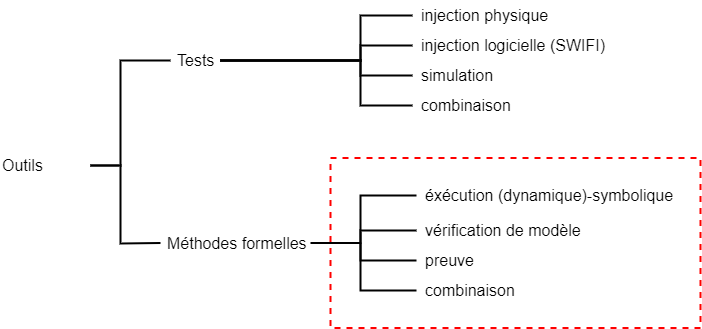
\includegraphics[scale=.45]{ch2-background/img/plan-soa-tools-formal.drawio.png}
              \caption{Outils basés sur les méthodes formelles}
              \label{fig:soa-tools-scheme-plan}
            \end{figure}
                
            La figure \ref{fig:soa-tools-scheme-plan} est un rappel du plan de la section \ref{sec:soa-tools} mettant en évidence les approches basées sur les méthodes formelles. 
            Ces outils basés peuvent parfois être rapprochés des techniques de simulation, dans le sens où le système n'est pas exécuté directement sur le matériel, mais analysé statiquement. C'est le cas pour l'exécution symbolique où le moteur d'exécution simule une exécution (ou plus exactement un ensemble d'exécutions) dans un modèle donné.
            De la même manière, certaines approches se rapprochent des méthodes de types \gls{swifi}, lorsque l'effet des fautes est mis en place dans le programme ou sa représentation, afin d'être fournies à un outil d'analyse formelle n'ayant pas de représentation pour les fautes \cite{Potet/ICST14, Le/DATE18}. 
            Les analyses formelles peuvent être appliquées à différents niveaux de représentation, en allant du niveau source aux représentations bas niveau comme le \gls{rtl} ou la spécification du circuit par exemple.             
            
            \paragraph{} 
            En 2007, Larsson et al. \cite{Larsson/VERIFY07} proposent une méthode appelée \textit{symbolic fault injection}. Ils présentent un outil d'analyse dans le cadre de la tolérance au fautes d'un programme source en Java et qui se base sur l'analyse formelle et l'exécution symbolique.
            Une instruction spécifique \texttt{inject(location);} est utilisée afin de spécifier que la zone mémoire \texttt{location} (variable, attribut etc.) peut être fautée. Leur implémentation utilise un modèle de bit flip sur les données et repose sur l'outil Key \cite{Ahrendt/Springer05}, une plateforme d'analyse formelle pour Java qui propose des fonctionnalités pour la vérification statique étendue, l'exécution symbolique, la vérification déductive et la spécification formelle.
            Des règles spécifiques ont été ajoutées dans Key pour simuler l'effet d'une faute dans l'état symbolique du programme.
            L'outil n'est cependant pas totalement automatique puisque l'utilisateur est sollicité pour spécifier les invariants de boucles par exemple.
            
            \textit{SymplFIED} \cite{Pattabiraman/DSN08}, est un outil d'évaluation reposant sur l'exécution symbolique et le model checking \cite{Pattabiraman/TC12}.
            L'outil prend en entrée un modèle de faute et un programme en assembleur qu'il transforme en un langage assembleur générique de type \gls{risc}.
            Cette représentation est implémentée avec le système Maude \cite{Clavel/ENTCS96, clavel2002maude} qui est un outil permettant la vérification de propriété sur un modèle et qui se base sur la \textit{rewritting logic}.
            SymplFIED supporte les fautes transitoires de un ou plusieurs bits dans le décodeur d'instruction, l'unité de calcul, les bus d'adresses et de données ou encore le fetch d'instruction, en faute unique.
            L'outil définit une procédure de modélisation de chaque type de faute sur le modèle machine dans Maude ainsi que des règles de propagation des erreurs entre les différents modules modélisés. Une erreur est représentée par un symbole \texttt{err} qui est propagé au fur et à mesure de l'exécution symbolique du programme.
            En plus de cela, l'outil vise à énumérer les cas d'erreurs qui ne sont pas détectées par des \textit{détecteurs}.
            La modélisation dans Maude fait quelques hypothèses comme l'absence d'erreur dans les détecteurs ou le fait que tout accès à une mémoire non initialisée donnera lieu à une exception et certaines opérations comme la multiplication ne sont pas exécutées symboliquement \cite{Pattabiraman/TC12}. 
            
            \textit{Lazart} \cite{Potet/ICST14} est un outil d'analyse de robustesse de programme sur la plateforme \gls{llvm} qui repose sur l'exécution symbolique effectuée par l'outil KLEE \cite{Cadar/OSDI08}. Lazart propose le modèle de l'inversion de test et chaque faute possible dans le programme est représentée par un booléen symbolique ce qui permet de générer les différents chemins d'attaque. 
            L'objectif d'attaque est défini à l'aide d'une propriété d'atteignabilité (par exemple le bloc d'authentification dans le programme \texttt{verify\_pin}) et les auteurs utilisent un algorithme de coloration de graphe pour réduire l'espace des fautes injectées (en ne considérant que les fautes sur les branches qui peuvent atteindre le bloc de base visé). 
            La dernière version (version 4) de Lazart est l'objet des chapitres \ref{chpt:lazart} et \ref{chpt:lazart-implem}. 
            
            En 2018, Le et al \cite{Le/DATE18} proposent aussi un outil reposant sur l'exécution symbolique au niveau \gls{llvm} utilisant KLEE.
            En ce sens, il ressemble à Lazart à la différence qu'il se concentre sur la tolérance aux fautes, c'est-à-dire avec un modèle bit-flip en simple faute qui vise le registre de calcul virtuel de \gls{llvm} ainsi que l'instruction \texttt{load}.
            Ils utilisent une version légèrement modifiée de KLEE dans la fonctionnalité permettant de démarrer l'exécution symbolique avec une \textit{graine} de manière à ne considérer que les chemins dans lesquelles l'injection d'une faute est possible.
            L'outil propose d'activer et désactiver l'injection localement ou globalement à l'aide de fonctions fournies dans une bibliothèque C qui est liée au programme à analyser.
            
            \begin{table}[h]
                {\tiny
                \begin{center}
                \setlength\tabcolsep{2.6pt}
                    \begin{tabular}{|l|l|l|l|l|l|l|l|l|l|}
                    \hline
                    Outil & Niveau & FA & Mode & Modèle & Fautes & Oracle & Technique & Mode & PAE \\ \hline
                    \begin{tabular}[c]{@{}l@{}}Larsson et al.\\ \cite{Larsson/VERIFY07}\end{tabular} & Source (Java) & Non & Interne & flip & 1 & \begin{tabular}[c]{@{}l@{}}propriété\\ logique\end{tabular} & \begin{tabular}[c]{@{}l@{}}MC + SE \\ (Key)\end{tabular} & Interne & Elevé \\ \hline
                    \begin{tabular}[c]{@{}l@{}}Symplified\\ \cite{Pattabiraman/DSN08}\end{tabular} & ASM (MISP) & Non & Interne & \begin{tabular}[c]{@{}l@{}}data (decoder,\\ bus, reg, mem)\end{tabular} & 1 & SDC & \begin{tabular}[c]{@{}l@{}}rewriting \\ logic + SE\\ (Maude)\end{tabular} & Interne & Elevé \\ \hline
                    \begin{tabular}[c]{@{}l@{}}Lazart\\ \cite{Potet/ICST14}\end{tabular} & LLVM & Oui & Externe & TI & X & logiciel & DSE (KLEE) & Externe & variable \\ \hline
                    \begin{tabular}[c]{@{}l@{}}Le et al.\\ \cite{Le/DATE18}\end{tabular} & LLVM & Non & Externe & \begin{tabular}[c]{@{}l@{}}bit-flip (reg.,\\ op.)\end{tabular} & 1 & logiciel & DSE (KLEE) & Externe & variable \\ \hline
                    \end{tabular}
                \end{center}
                }            
                \caption{Comparaison de quelques outils reposant sur l'analyse formelle
                \label{tbl:tools-formal}}
            \end{table}
            
            La table \ref{tbl:tools-formal} présente une table de comparaison d'outils basés sur l'analyse formelle.
            Les colonnes \textit{Niveau}, \textit{FA}, \textit{Modèle}, \textit{Faute} et \textit{Oracle} sont équivalentes à celles des tables précédentes.
            La colonne \textit{Mode} précise si l'outil utilise de façon externe un outil d'analyse formelle en instrumentant le code à la manière d'un outil \gls{swifi}.
            La colonne technique liste les méthodes formelles utilisées par l'outil.
            La colonne \textit{PAE} correspond au passage à l'échelle de l'outil.
            
            \begin{figure}[hbt]\centering
              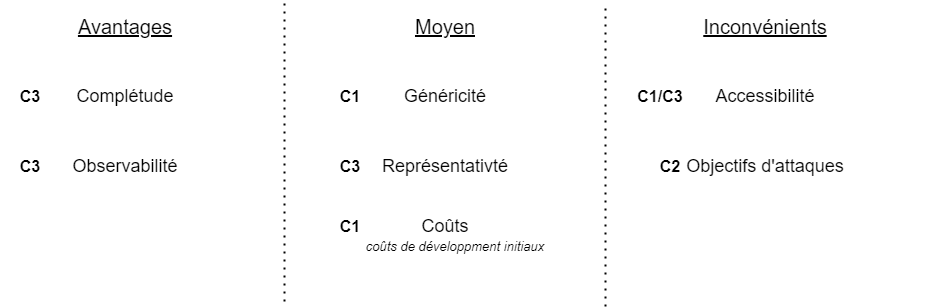
\includegraphics[scale=.43]{ch2-background/img/advantages-formal.drawio.png}
              \caption{Caractéristiques des méthodes formelles}
              \label{fig:soa-tools-scheme-formal}
            \end{figure}
            
            La figure \ref{fig:soa-tools-scheme-simu} présente les caractéristiques des outils basés sur les méthodes formelles.
            Les méthodes formelles ont un avantage en ce qui concerne la complétude des résultats, dépendant de la technique utilisée. 
            Ces approches étant appliquées à des niveaux variés d'abstraction, et donc de modèles de faute, la représentativité des
            résultats est très variable.
            La performance n'est pas réellement comparable par rapport aux outils basés sur les tests, puisque tous les chemins et toutes les combinaisons de fautes sont potentiellement explorés, mais certains outils souffrent d'un problème de passage à l'échelle, corrélé à la méthode formelle utilisée.
            L'accessibilité et l'automatisation ne sont pas toujours bons pour ces outils, demandant parfois une expertise de l'utilisateur dans la méthode formelle utilisée ou bien une intervention importante de la part de l'utilisateur \cite{Larsson/VERIFY07}.
    
        \subsection{Conclusion}
        \label{sec:soa-tools-conclusion}
            
            Des approches très variées ont été proposées pour l'évaluation de la robustesse dans le cadre de l'injection de fautes, comme l'ont montré les sections précédentes.
            
                \begin{table}[h]
                    {\small
                    \begin{center}
                    \setlength\tabcolsep{3.5pt}
                        \begin{tabular}{|l|c|c|c|c|}
                        \hline
                        Méthode & Mise-en-place & Représentativité & Reproductibilité & Observabilité  \\ \hline
                        Injection Physique & Très élevé & Très élevé & Faible - Elevé & Faible  \\ \hline
                        SWIFI & Faible & Faible - élevé & Moyen & Moyen  \\ \hline
                        Simulation & Faible elevé & Moyen - élevé & Elevé & Elevé - Très élevé  \\ \hline
                        Méthodes formelles & Faible - Elevé & Moyen - élevé & Moyen - elevé & Elevé - Très élevé  \\ \hline
                        \end{tabular}
                        
                        \vspace{0.2cm}
                        
                        \begin{tabular}{|l|c|c|c|c|c|}
                        \hline
                        Méthode & Contexte  & Complétude & Accessibilité & Généricité & Contexte \\ \hline
                        Inj Physique & Varié &Faible & Faible & Faible & Varié \\ \hline
                        Swifi & Varié & Faible & Moyen & Elevée & Varié \\ \hline
                        Simu & Varié & Faible & Moyen & Moyen - élevé & Varié \\ \hline
                        Formal & Limité & Elevé - Très élevé & Faible & Moyen - élevé & Limité \\ \hline
                        \end{tabular}
                    \end{center}
                    }           
                    \caption{Comparaison des méthodes d'analyse de robustesse contre les fautes \label{tbl:tools-conclusion}}
                \end{table}
            
            La table \ref{tbl:tools-conclusion} compare les caractéristiques de la section \ref{sec:soa-tools-carac} pour les différentes techniques d'analyse présentées dans les sections précédentes.
            Chaque valeur correspond à une pondération entre \textit{faible}, \textit{moyen}, \textit{élevé} et \textit{très élevé}, visant à préserver les rapports entre les classes de techniques d'analyse ainsi que les variations au sein d'une même classe.
            
            Les méthodes formelles ont un très net avantage en ce qui concerne la couverture des exécutions fautées, mais certaines techniques comme l'exécution symbolique souffrent de l'explosion combinatoire induite par les fautes pour le passage à l'échelle, en particulier dans un contexte multi-fautes.
            De plus, certaines propriétés et objectif d'attaque peuvent être difficiles à exprimer ou à analyser avec certaines approches formelles, notamment les propriétés basées sur la comparaisons de traces (canaux-auxiliaires) qui peuvent être plus simples à évaluer avec un golden run. 
            La simulation offre des avantages en termes de contrôlabilité.
            Les méthodes de type \gls{swifi} sont généralement les plus faciles à mettre en place.
            
            Certaines caractéristiques dépendent fortement des choix de conception et d'implémentation de l'outil. Si la contrôlabilité est difficile dans le cadre de l'injection physique, cette caractéristique dépend surtout de ce que l'outil met à disposition à l'utilisateur pour les autres classes d'outils, les outils simulant un système (que ce soit dans un simulateur ou par une modélisation formelle) étant aussi avantagés. 
            L'accessibilité est un bon exemple de caractéristique dépendant en grande partie de l'outil plus que de la méthode utilisée, qu'il s'agisse d'automatisation, de contrôlabilité ou d'expertise. 
            
            D'autres caractéristiques dépendent aussi fortement du niveau de représentation considéré par l'outil, qui peut être très variable au sein des outils d'une même méthode d'analyse. 
            Dans ce cas, le niveau de représentation de l'outil influe directement sur la représentativité, les modèles de faute supportés et la généricité de l'outil.
            
            L'outil Lazart, qui est l'objet du chapitre suivant, est un outil d'analyse formelle utilisant l'exécution dynamique-symbolique.
            Lazart utilise l'outil KLEE qui effectue une exécution dynamique-symbolique sur le code \gls{llvm} et peut ainsi être vu comme un simulateur utilisant un modèle mémoire et une représentation du système particuliers.
            Les fautes sont introduites par une mutation du programme fourni à KLEE, correspondant à ce qui existe dans le cadre des outils \gls{swifi} au niveau \gls{llvm}.
            
            Lazart vise à répondre à certaines problématiques tirées de cette section en ce qui concerne ce type d'outils reposant sur les méthodes formelle ainsi que l'émulation des fautes au niveau logiciel.
            
            \begin{itemize}
                \item \textit{Performance} et \textit{passage à l'échelle}: maîtriser le multi-fautes et l'explosion combinatoire engendrée.
                \item \textit{Représentativité}: limiter la perte de représentativité liée à la sur-couche de l'émulation des fautes.
                \item \textit{Accessibilité} et \textit{généricité}: limiter le niveau d'expertise requis pour l'utilisation de l'outil et laisser une contrôlabilité élevée à l'utilisateur.
            \end{itemize}
            
            Les contributions de Lazart visent ainsi à proposer des solutions pour ces problématiques:
            \begin{itemize}
                \item Support de l'inter-procédural et de la combinaison de modèles de faute ainsi qu'une description à grain fin des fautes par l'utilisateur (\textit{représentativité} et \textit{contrôlabilité}).
                \item Une \gls{api} Python facilitant la description des analyses et la présentation des résultats (\textit{accessibilité}).
                \item Une analyse plus fine des résultats produits.
            \end{itemize}
    
    